\documentclass[11pt]{book}
\usepackage{amsmath}
\usepackage{amsfonts}
\usepackage{amssymb}
\usepackage{geometry}
\geometry{a4paper, margin=1in}
\usepackage{graphicx}
\usepackage[hidelinks]{hyperref}
\usepackage{amsthm}
\usepackage{tikz}
\usepackage{subcaption}
\usetikzlibrary{positioning}
\usepackage{pgfplots} 
\usepackage[ruled,vlined]{algorithm2e} 
\usepackage{dsfont}
\usepackage{graphicx}
\usepackage{mathdesign}
\usepackage{float}
\usepackage{todonotes} 
\usepackage{empheq}
\usepackage{array}
\usepackage[ruled,vlined]{algorithm2e} 



\setlength{\parindent}{0pt}


\newcommand\mycommfont[1]{\footnotesize\ttfamily\textcolor{blue}{#1}}
\newcommand\defeq{\stackrel{\mathclap{\normalfont\mbox{def}}}{=}}
\SetCommentSty{mycommfont}

\DeclareMathOperator*{\argmax}{argmax}
\DeclareMathOperator*{\argmin}{argmin}

\newtheorem{theorem}{Theorem}[section]
\newtheorem{lemma}{Lemma}[section]
\newtheorem{definition}{Definition}[section]
\newtheorem{corollary}{Corollary}[section]
\newtheorem{claim}{claim}[section]
\newtheorem{example}{Example}[section]


\newtheorem*{claim*}{Claim}
\newtheorem*{lemma*}{Lemma}
\newtheorem*{corollary*}{Corollary}
\newtheorem*{remark*}{Remark}
\newtheorem*{example*}{Example}
\newtheorem*{examples*}{Examples}
\newtheorem*{definition*}{Definition}



\setcounter{tocdepth}{3}





\begin{document}

\begin{titlepage}
    \begin{center}
     {\huge\bfseries 
     Intro To Optimization \\
     }
     % ----------------------------------------------------------------
     \vspace{1.5cm}
     {\Large\bfseries Hadar Tal}\\[5pt]
     hadar.tal@mail.huji.ac.il\\[14pt]
      % ----------------------------------------------------------------
     \vspace{2cm}
     {This paper is a summary of the educational materials and lectures from 
     \begin{itemize}
        \item \textbf{Optimization for Computer Science} by Professor Tomer Koren, Tel Aviv University
        \item \textbf{Wikipedia}
        \item \textbf{3Blue1Brown} YouTube channel
     \end{itemize}
     }

     \vfill
    {Winter 2024}
    \end{center}
\end{titlepage}


\frontmatter
\tableofcontents

% * * * * * * * * * * * * * * * * * * * * * * * * 
% * * * * * * * * * * * * * * * * * * * * * * * * 
% * * * * * * * * * * * * * * * * * * * * * * * * 
% * * * * * * * * * * * * * * * * * * * * * * * * 
% * * * * * * * * * * * * * * * * * * * * * * * * 
% * * * * * * * * * * * * * * * * * * * * * * * * 
% * * * * * * * * * * * * * * * * * * * * * * * * 
% * * * * * * * * * * * * * * * * * * * * * * * * 
% * * * * * * * * * * * * * * * * * * * * * * * * 
% * * * * * * * * * * * * * * * * * * * * * * * * 
% * * * * * * * * * * * * * * * * * * * * * * * * 
% * * * * * * * * * * * * * * * * * * * * * * * * 
% * * * * * * * * * * * * * * * * * * * * * * * * 
% * * * * * * * * * * * * * * * * * * * * * * * * 
% * * * * * * * * * * * * * * * * * * * * * * * * 
% * * * * * * * * * * * * * * * * * * * * * * * * 
% * * * * * * * * * * * * * * * * * * * * * * * * 
% * * * * * * * * * * * * * * * * * * * * * * * * 
% * * * * * * * * * * * * * * * * * * * * * * * * 

\mainmatter

\chapter{Linear Programming (LP)}

\begin{definition}(The Primal Problem in canonical form) \\
    The primal problem in canonical form is given by
    \begin{equation}
        \begin{aligned}
            \text{maximize} \quad & \langle c,x \rangle \\
            \text{subject to} \quad & Ax \leq b \\
            & x \geq 0
        \end{aligned}
    \end{equation}
\end{definition}


\begin{definition}(The Primal Problem in standard form) \\
    The primal problem in standard form is given by
    \begin{equation}
        \begin{aligned}
            \text{maximize} \quad & \langle c,x \rangle \\
            \text{subject to} \quad & Ax = b \\
            & x \geq 0
        \end{aligned}
    \end{equation}
\end{definition}

\begin{definition}(The Dual Problem in canonical form) \\
    The dual problem in canonical form is given by
    \begin{equation}
        \begin{aligned}
            \text{minimize} \quad & \langle b,y \rangle \\
            \text{subject to} \quad & A^T y \geq c \\
            & y \geq 0
        \end{aligned}
    \end{equation}
\end{definition}


\begin{theorem}(Weak Duality) \\
    Let $x$ be a feasible solution to the primal problem and $y$ be a feasible solution to the dual problem. Then
    \begin{equation}
        \langle c,x \rangle \leq \langle b,y \rangle
    \end{equation}
\end{theorem}

\begin{theorem}(Strong Duality) \\
    If the primal problem has an optimal solution, then the dual problem also has an optimal solution and the optimal values of the primal and dual problems are equal.
\end{theorem}



\section{Minimiax Theorem}

\subsection{Theorem}
Let \(X \subset \mathbb{R}^n\) and \(Y \subset \mathbb{R}^m\) be compact convex sets. If \(f : X \times Y \rightarrow \mathbb{R}\) is a continuous function that is concave-convex, i.e.,
\begin{itemize}
    \item \(f(\cdot, y) : X \rightarrow \mathbb{R}\) is concave for fixed \(y\),
    \item \(f(x, \cdot) : Y \rightarrow \mathbb{R}\) is convex for fixed \(x\),
\end{itemize}
then we have that
\[
\max_{x \in X} \min_{y \in Y} f(x, y) = \min_{y \in Y} \max_{x \in X} f(x, y).
\]

\subsection{Special Case: Bilinear Function}
The theorem holds in particular if \(f(x, y)\) is a linear function in both of its arguments (and therefore is bilinear) since a linear function is both concave and convex. Thus, if \(f(x, y) = x^T Ay\) for a finite matrix \(A \in \mathbb{R}^{n \times m}\), we have:
\[
\max_{x \in X} \min_{y \in Y} x^T Ay = \min_{y \in Y} \max_{x \in X} x^T Ay.
\]
The bilinear special case is particularly important for zero-sum games, when the strategy set of each player consists of lotteries over actions (mixed strategies), and payoffs are induced by expected value. In the above formulation, \(A\) is the payoff matrix.

The function \(f(x, y) = y^2 - x^2\) is shown below as an example of a concave-convex function.

\begin{figure}[H]
    \centering
    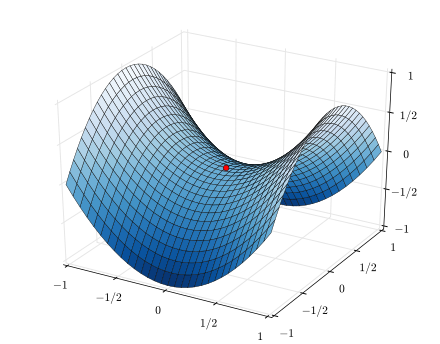
\includegraphics[width=0.5\textwidth]{Figs/Saddle_point.png}
    \caption{Concave-convex function}
\end{figure}



% * * * * * * * * * * * * * * * * * * * * * * * * * * * * * * * * * * * * * * * * * * * * * * * *
% * * * * * * * * * * * * * * * * * * * * * * * * * * * * * * * * * * * * * * * * * * * * * * * *
% * * * * * * * * * * * * * * * * * * * * * * * * * * * * * * * * * * * * * * * * * * * * * * * *
% * * * * * * * * * * * * * * * * * * * * * * * * * * * * * * * * * * * * * * * * * * * * * * * *
% * * * * * * * * * * * * * * * * * * * * * * * * * * * * * * * * * * * * * * * * * * * * * * * *
% * * * * * * * * * * * * * * * * * * * * * * * * * * * * * * * * * * * * * * * * * * * * * * * *
% * * * * * * * * * * * * * * * * * * * * * * * * * * * * * * * * * * * * * * * * * * * * * * * *
% * * * * * * * * * * * * * * * * * * * * * * * * * * * * * * * * * * * * * * * * * * * * * * * *
% * * * * * * * * * * * * * * * * * * * * * * * * * * * * * * * * * * * * * * * * * * * * * * * *
% * * * * * * * * * * * * * * * * * * * * * * * * * * * * * * * * * * * * * * * * * * * * * * * *
% * * * * * * * * * * * * * * * * * * * * * * * * * * * * * * * * * * * * * * * * * * * * * * * *
% * * * * * * * * * * * * * * * * * * * * * * * * * * * * * * * * * * * * * * * * * * * * * * * *
% * * * * * * * * * * * * * * * * * * * * * * * * * * * * * * * * * * * * * * * * * * * * * * * *
% * * * * * * * * * * * * * * * * * * * * * * * * * * * * * * * * * * * * * * * * * * * * * * * *
% * * * * * * * * * * * * * * * * * * * * * * * * * * * * * * * * * * * * * * * * * * * * * * * *
% * * * * * * * * * * * * * * * * * * * * * * * * * * * * * * * * * * * * * * * * * * * * * * * *
% * * * * * * * * * * * * * * * * * * * * * * * * * * * * * * * * * * * * * * * * * * * * * * * *
% * * * * * * * * * * * * * * * * * * * * * * * * * * * * * * * * * * * * * * * * * * * * * * * *
% * * * * * * * * * * * * * * * * * * * * * * * * * * * * * * * * * * * * * * * * * * * * * * * *
% * * * * * * * * * * * * * * * * * * * * * * * * * * * * * * * * * * * * * * * * * * * * * * * *
% * * * * * * * * * * * * * * * * * * * * * * * * * * * * * * * * * * * * * * * * * * * * * * * *
\chapter{Important subsets of $\mathbb{R}^n$}

\begin{definition}{Open set} \\
A set $S \subseteq \mathbb{R}^n$ is open if for all $x \in S$, there exists $\epsilon > 0$ such that $B(x, \epsilon) \subseteq S$.
\end{definition}

\begin{definition}{Closed set} \\
A set $S \subseteq \mathbb{R}^n$ is closed if its complement is open.
\end{definition}

\begin{definition}{Interior point} \\
A point $x \in S$ is an interior point of $S$ if there exists $\epsilon > 0$ such that $B(x, \epsilon) \subseteq S$.
\end{definition}

\begin{corollary}{Open set characterization} \\
A set $S \subseteq \mathbb{R}^n$ is open if and only if every point in $S$ is an interior point of $S$.
\end{corollary}

\begin{definition}{Boundary point} \\
A point $x \in S$ is a boundary point of $S$ if for all $\epsilon > 0$, $B(x, \epsilon) \cap S \neq \emptyset$ and $B(x, \epsilon) \cap S^c \neq \emptyset$.
\end{definition}

\begin{definition}{Half-space} \\
A half-space in $\mathbb{R}^n$ is a set of the form $\{x \in \mathbb{R}^n : a^T x \leq b\}$ for some $a \in \mathbb{R}^n$ and $b \in \mathbb{R}$.
\end{definition}

\begin{definition}{Hyperplane} \\
A hyperplane in $\mathbb{R}^n$ is a set of the form $\{x \in \mathbb{R}^n : a^T x = b\}$ for some $a \in \mathbb{R}^n$ and $b \in \mathbb{R}$.
\end{definition}

\begin{definition}{Polyhedron (Polyhedra)} \\
A polyhedron in $\mathbb{R}^n$ is a set of the form $\{x \in \mathbb{R}^n : Ax \leq b\}$ for some $A \in \mathbb{R}^{m \times n}$ and $b \in \mathbb{R}^m$.
Equivalently, a polyhedron is the intersection of finitely many half-spaces.
\end{definition}

\begin{definition}{Polytope} \\
A polytope in $\mathbb{R}^n$ is a bounded polyhedron - i.e., there exists $r > 0$ such that $\forall x \in \{x \in \mathbb{R}^n : Ax \leq b\} \implies ||x|| \leq r$.
Equivalently, a polytope is the convex hull of finitely many points.
\end{definition}

\begin{figure}[H]
    \centering
    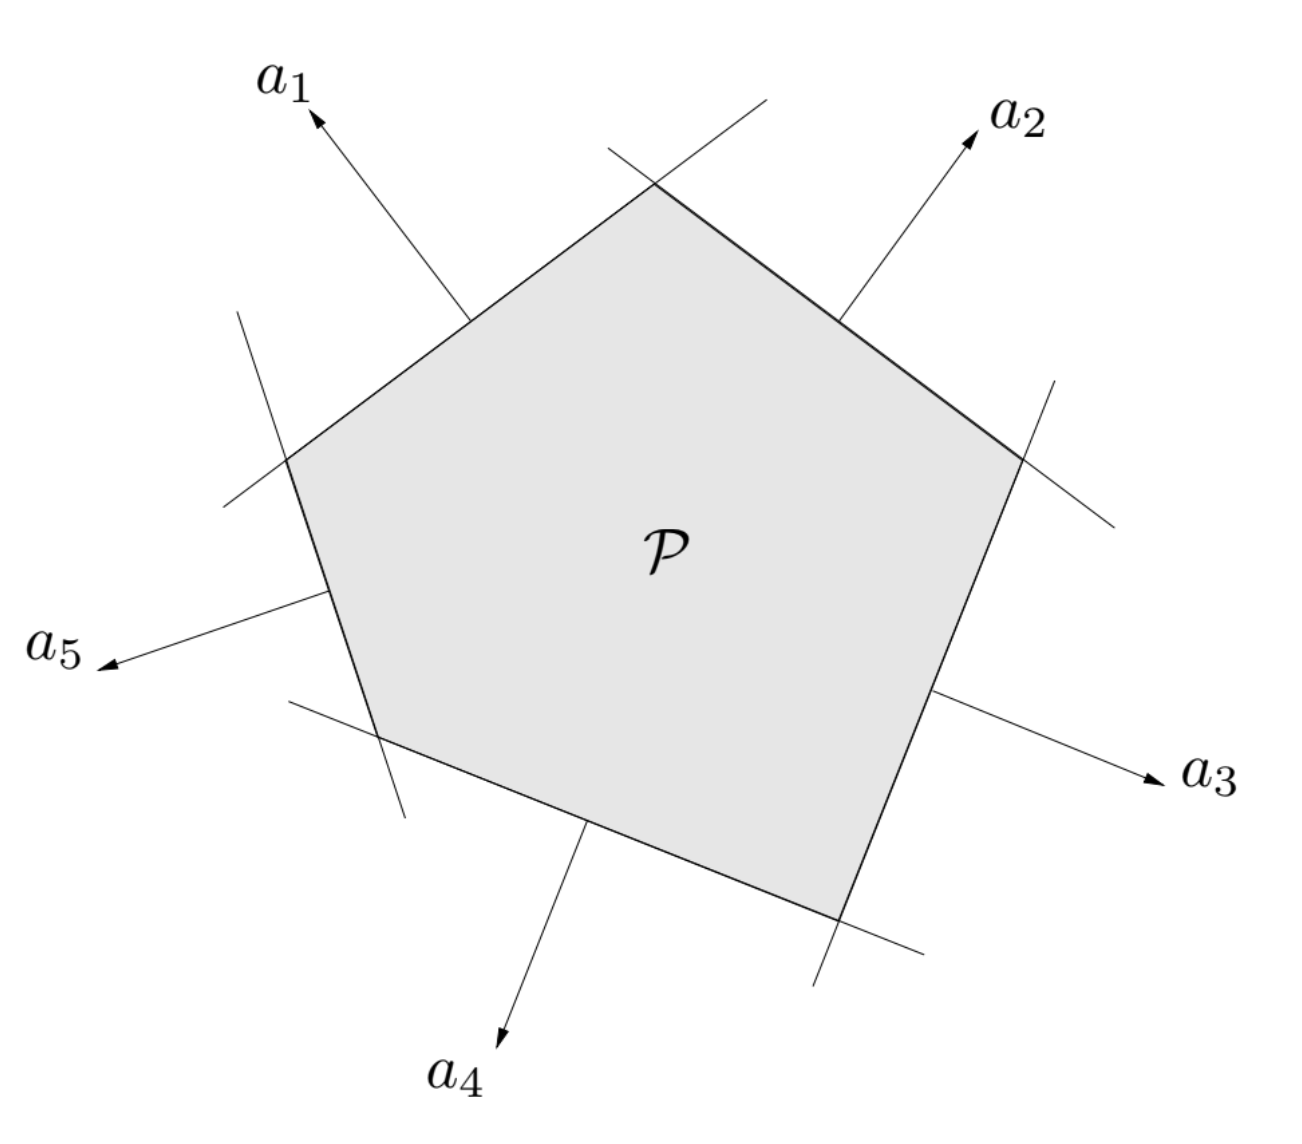
\includegraphics[width=0.3\textwidth]{Figs/polyhedron.png}
    \caption{Polytope}
\end{figure}

\begin{definition}{Convex set} \\
    A set $S \subseteq \mathbb{R}^n$ is convex if for all $x,y \in S$ and $\lambda \in [0,1]$, we have $\lambda t + (1- \lambda)y \in S$.
\end{definition}    

\begin{figure}[H]
    \centering
    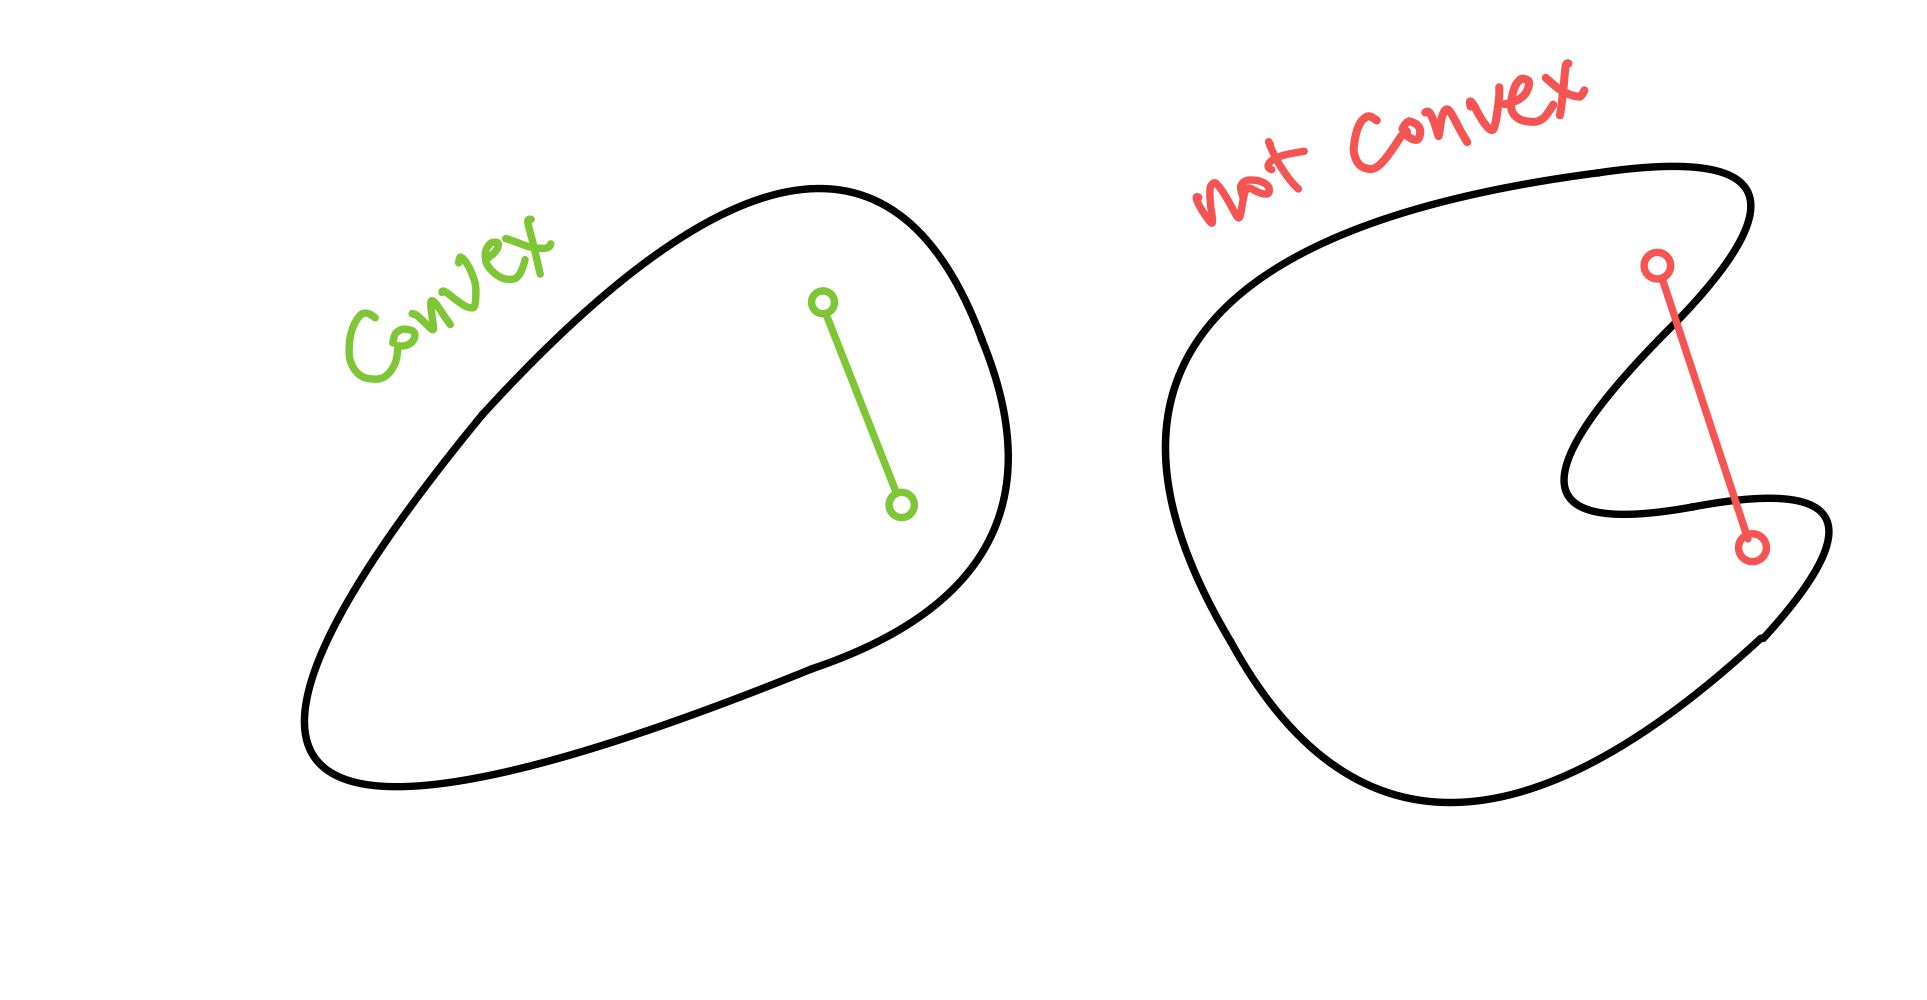
\includegraphics[width=0.5\textwidth]{Figs/convex_set.png}
    \caption{Convex set}
\end{figure}

\begin{definition}{Convex hull} \\
The convex hull of a set $S \subseteq \mathbb{R}^n$ is the smallest convex set that contains $S$.
\end{definition}


\begin{definition}{Conic combination} \\
A point $x \in \mathbb{R}^n$ is a conic combination of $y_1, \ldots, y_k \in \mathbb{R}^n$ 
if there exist $\lambda_1, \ldots, \lambda_k \geq 0$ such that $x = \sum_{i=1}^k \lambda_i y_i$.    
\end{definition}

\begin{definition}{Conic hull} \\
The conic hull of a finite set $S \subseteq \mathbb{R}^n$ is the set of all conic combinations of points in $S$.
\end{definition}


\begin{definition}{Convex cone} \\
A set $S \subseteq \mathbb{R}^n$ is a convex cone if for all $x \in S$ and $\lambda \geq 0$, we have $\lambda x \in S$.
\end{definition}

\begin{figure}[H]
    \begin{subfigure}{0.5\textwidth}
        \centering
        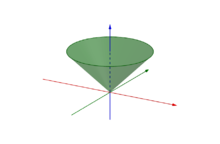
\includegraphics[width=\linewidth]{Figs/circular-pyramid.png}
        \caption{Convex cone that is not a conic hull of finitely many generators.}
    \end{subfigure}
    \begin{subfigure}{0.5\textwidth}
        \centering
        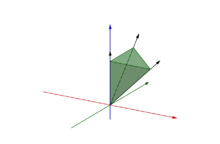
\includegraphics[width=\linewidth]{Figs/polyhedral_cone.png}
        \caption{Convex cone genrated by the conic combination of three black vectors (conic hull).}
    \end{subfigure}
\end{figure}

\begin{definition}{Normal cone} \\
The normal cone to a set $S$ at a point $x$ is defined as
\begin{equation}
    N_S(x) = \{ v \in \mathbb{R}^n : \langle v, y-x \rangle \leq 0 \text{ for all } y \in S \}
\end{equation}
\end{definition}

\begin{definition}{Tangent cone} \\
The tangent cone to a set $S$ at a point $x$ is defined as
\begin{equation}
    T_S(x) = \{ v \in \mathbb{R}^n : \lim_{t \rightarrow 0^+} \frac{x + tv - x}{t} \in S \}
\end{equation}
\end{definition}

\begin{figure}[H]
    \centering
    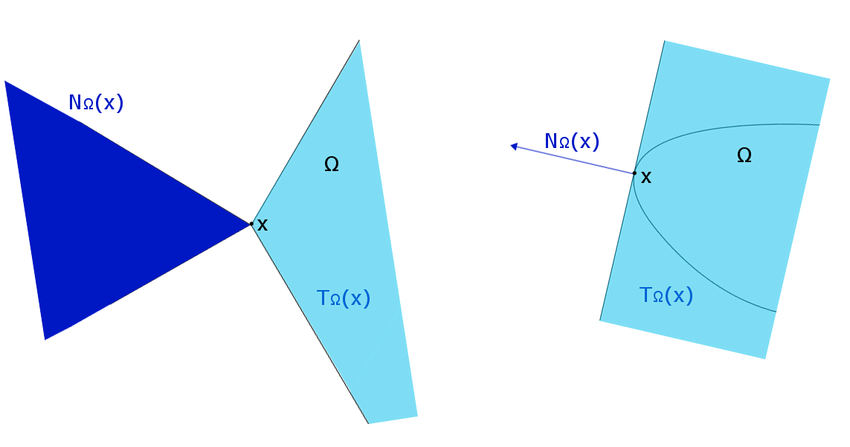
\includegraphics[width=0.5\textwidth]{Figs/normal-cones.png}
    \caption{Normal and tangent cones}
\end{figure}

\begin{theorem}{Normal cone of polyhedron} \\
The normal cone to a polyhedron $S = \{x \in \mathbb{R}^n : \forall j \in [m] \quad a_j \cdot x \leq b_j\}$ at a point $x$ is given by
\begin{equation}
    N_S(x) = \{ \sum_{j} \lambda_j a_j : \lambda_j \geq 0  \text{ and }  a_j \cdot x = b_j \}
\end{equation}
    
\end{theorem}


% * * * * * * * * * * * * * * * * * * * * * * * * * * * * * * * * * * * * * * * * * * * * * * * *
% * * * * * * * * * * * * * * * * * * * * * * * * * * * * * * * * * * * * * * * * * * * * * * * *
% * * * * * * * * * * * * * * * * * * * * * * * * * * * * * * * * * * * * * * * * * * * * * * * *
% * * * * * * * * * * * * * * * * * * * * * * * * * * * * * * * * * * * * * * * * * * * * * * * *
% * * * * * * * * * * * * * * * * * * * * * * * * * * * * * * * * * * * * * * * * * * * * * * * *
% * * * * * * * * * * * * * * * * * * * * * * * * * * * * * * * * * * * * * * * * * * * * * * * *
% * * * * * * * * * * * * * * * * * * * * * * * * * * * * * * * * * * * * * * * * * * * * * * * *
% * * * * * * * * * * * * * * * * * * * * * * * * * * * * * * * * * * * * * * * * * * * * * * * *
% * * * * * * * * * * * * * * * * * * * * * * * * * * * * * * * * * * * * * * * * * * * * * * * *
% * * * * * * * * * * * * * * * * * * * * * * * * * * * * * * * * * * * * * * * * * * * * * * * *
% * * * * * * * * * * * * * * * * * * * * * * * * * * * * * * * * * * * * * * * * * * * * * * * *
% * * * * * * * * * * * * * * * * * * * * * * * * * * * * * * * * * * * * * * * * * * * * * * * *
% * * * * * * * * * * * * * * * * * * * * * * * * * * * * * * * * * * * * * * * * * * * * * * * *
% * * * * * * * * * * * * * * * * * * * * * * * * * * * * * * * * * * * * * * * * * * * * * * * *
% * * * * * * * * * * * * * * * * * * * * * * * * * * * * * * * * * * * * * * * * * * * * * * * *
% * * * * * * * * * * * * * * * * * * * * * * * * * * * * * * * * * * * * * * * * * * * * * * * *
% * * * * * * * * * * * * * * * * * * * * * * * * * * * * * * * * * * * * * * * * * * * * * * * *
% * * * * * * * * * * * * * * * * * * * * * * * * * * * * * * * * * * * * * * * * * * * * * * * *
% * * * * * * * * * * * * * * * * * * * * * * * * * * * * * * * * * * * * * * * * * * * * * * * *
% * * * * * * * * * * * * * * * * * * * * * * * * * * * * * * * * * * * * * * * * * * * * * * * *
% * * * * * * * * * * * * * * * * * * * * * * * * * * * * * * * * * * * * * * * * * * * * * * * *


\chapter{Tractability and efficiency}

% * * * * * * * * * * * * * * * * * * * * * * * * * * * * * * * * * * * * * * * * * * * * * * * *
% * * * * * * * * * * * * * * * * * * * * * * * * * * * * * * * * * * * * * * * * * * * * * * * *
% * * * * * * * * * * * * * * * * * * * * * * * * * * * * * * * * * * * * * * * * * * * * * * * *
% * * * * * * * * * * * * * * * * * * * * * * * * * * * * * * * * * * * * * * * * * * * * * * * *
% * * * * * * * * * * * * * * * * * * * * * * * * * * * * * * * * * * * * * * * * * * * * * * * *
% * * * * * * * * * * * * * * * * * * * * * * * * * * * * * * * * * * * * * * * * * * * * * * * *
% * * * * * * * * * * * * * * * * * * * * * * * * * * * * * * * * * * * * * * * * * * * * * * * *
% * * * * * * * * * * * * * * * * * * * * * * * * * * * * * * * * * * * * * * * * * * * * * * * *
% * * * * * * * * * * * * * * * * * * * * * * * * * * * * * * * * * * * * * * * * * * * * * * * *
% * * * * * * * * * * * * * * * * * * * * * * * * * * * * * * * * * * * * * * * * * * * * * * * *
% * * * * * * * * * * * * * * * * * * * * * * * * * * * * * * * * * * * * * * * * * * * * * * * *
% * * * * * * * * * * * * * * * * * * * * * * * * * * * * * * * * * * * * * * * * * * * * * * * *
% * * * * * * * * * * * * * * * * * * * * * * * * * * * * * * * * * * * * * * * * * * * * * * * *
% * * * * * * * * * * * * * * * * * * * * * * * * * * * * * * * * * * * * * * * * * * * * * * * *
% * * * * * * * * * * * * * * * * * * * * * * * * * * * * * * * * * * * * * * * * * * * * * * * *
% * * * * * * * * * * * * * * * * * * * * * * * * * * * * * * * * * * * * * * * * * * * * * * * *
% * * * * * * * * * * * * * * * * * * * * * * * * * * * * * * * * * * * * * * * * * * * * * * * *
% * * * * * * * * * * * * * * * * * * * * * * * * * * * * * * * * * * * * * * * * * * * * * * * *
% * * * * * * * * * * * * * * * * * * * * * * * * * * * * * * * * * * * * * * * * * * * * * * * *
% * * * * * * * * * * * * * * * * * * * * * * * * * * * * * * * * * * * * * * * * * * * * * * * *
% * * * * * * * * * * * * * * * * * * * * * * * * * * * * * * * * * * * * * * * * * * * * * * * *

\chapter{Convexity}

% * * * * * * * * * * * * * * * * * * * * * * * * * * * * * * * * * * * * * * * * * * * * * * * *
% * * * * * * * * * * * * * * * * * * * * * * * * * * * * * * * * * * * * * * * * * * * * * * * *
% * * * * * * * * * * * * * * * * * * * * * * * * * * * * * * * * * * * * * * * * * * * * * * * *
% * * * * * * * * * * * * * * * * * * * * * * * * * * * * * * * * * * * * * * * * * * * * * * * *
% * * * * * * * * * * * * * * * * * * * * * * * * * * * * * * * * * * * * * * * * * * * * * * * *
% * * * * * * * * * * * * * * * * * * * * * * * * * * * * * * * * * * * * * * * * * * * * * * * *
% * * * * * * * * * * * * * * * * * * * * * * * * * * * * * * * * * * * * * * * * * * * * * * * *
% * * * * * * * * * * * * * * * * * * * * * * * * * * * * * * * * * * * * * * * * * * * * * * * *
% * * * * * * * * * * * * * * * * * * * * * * * * * * * * * * * * * * * * * * * * * * * * * * * *
% * * * * * * * * * * * * * * * * * * * * * * * * * * * * * * * * * * * * * * * * * * * * * * * *
% * * * * * * * * * * * * * * * * * * * * * * * * * * * * * * * * * * * * * * * * * * * * * * * *
% * * * * * * * * * * * * * * * * * * * * * * * * * * * * * * * * * * * * * * * * * * * * * * * *
% * * * * * * * * * * * * * * * * * * * * * * * * * * * * * * * * * * * * * * * * * * * * * * * *
% * * * * * * * * * * * * * * * * * * * * * * * * * * * * * * * * * * * * * * * * * * * * * * * *
% * * * * * * * * * * * * * * * * * * * * * * * * * * * * * * * * * * * * * * * * * * * * * * * *
% * * * * * * * * * * * * * * * * * * * * * * * * * * * * * * * * * * * * * * * * * * * * * * * *
% * * * * * * * * * * * * * * * * * * * * * * * * * * * * * * * * * * * * * * * * * * * * * * * *
% * * * * * * * * * * * * * * * * * * * * * * * * * * * * * * * * * * * * * * * * * * * * * * * *
% * * * * * * * * * * * * * * * * * * * * * * * * * * * * * * * * * * * * * * * * * * * * * * * *
% * * * * * * * * * * * * * * * * * * * * * * * * * * * * * * * * * * * * * * * * * * * * * * * *
% * * * * * * * * * * * * * * * * * * * * * * * * * * * * * * * * * * * * * * * * * * * * * * * *

\chapter{Basic Gradient Methods}

% * * * * * * * * * * * * * * * * * * * * * * * * * * * * * * * * * * * * * * * * * * * * * * * *
% * * * * * * * * * * * * * * * * * * * * * * * * * * * * * * * * * * * * * * * * * * * * * * * *
% * * * * * * * * * * * * * * * * * * * * * * * * * * * * * * * * * * * * * * * * * * * * * * * *
% * * * * * * * * * * * * * * * * * * * * * * * * * * * * * * * * * * * * * * * * * * * * * * * *
% * * * * * * * * * * * * * * * * * * * * * * * * * * * * * * * * * * * * * * * * * * * * * * * *
% * * * * * * * * * * * * * * * * * * * * * * * * * * * * * * * * * * * * * * * * * * * * * * * *
% * * * * * * * * * * * * * * * * * * * * * * * * * * * * * * * * * * * * * * * * * * * * * * * *
% * * * * * * * * * * * * * * * * * * * * * * * * * * * * * * * * * * * * * * * * * * * * * * * *
% * * * * * * * * * * * * * * * * * * * * * * * * * * * * * * * * * * * * * * * * * * * * * * * *
% * * * * * * * * * * * * * * * * * * * * * * * * * * * * * * * * * * * * * * * * * * * * * * * *
% * * * * * * * * * * * * * * * * * * * * * * * * * * * * * * * * * * * * * * * * * * * * * * * *
% * * * * * * * * * * * * * * * * * * * * * * * * * * * * * * * * * * * * * * * * * * * * * * * *
% * * * * * * * * * * * * * * * * * * * * * * * * * * * * * * * * * * * * * * * * * * * * * * * *
% * * * * * * * * * * * * * * * * * * * * * * * * * * * * * * * * * * * * * * * * * * * * * * * *
% * * * * * * * * * * * * * * * * * * * * * * * * * * * * * * * * * * * * * * * * * * * * * * * *
% * * * * * * * * * * * * * * * * * * * * * * * * * * * * * * * * * * * * * * * * * * * * * * * *
% * * * * * * * * * * * * * * * * * * * * * * * * * * * * * * * * * * * * * * * * * * * * * * * *
% * * * * * * * * * * * * * * * * * * * * * * * * * * * * * * * * * * * * * * * * * * * * * * * *
% * * * * * * * * * * * * * * * * * * * * * * * * * * * * * * * * * * * * * * * * * * * * * * * *
% * * * * * * * * * * * * * * * * * * * * * * * * * * * * * * * * * * * * * * * * * * * * * * * *
% * * * * * * * * * * * * * * * * * * * * * * * * * * * * * * * * * * * * * * * * * * * * * * * *

\chapter{Definitions and Fundamental Theorems}



\begin{definition} (Convex function): A function $f : S \rightarrow \mathbb{R}$ defined on a convex set $S$ is convex if, for all $x, y \in S$ and $\lambda \in [0,1]$, 
\[ f(\lambda x + (1-\lambda)y) \leq \lambda f(x) + (1-\lambda) f(y). \]
\end{definition}

\begin{figure}[H]
    \centering
    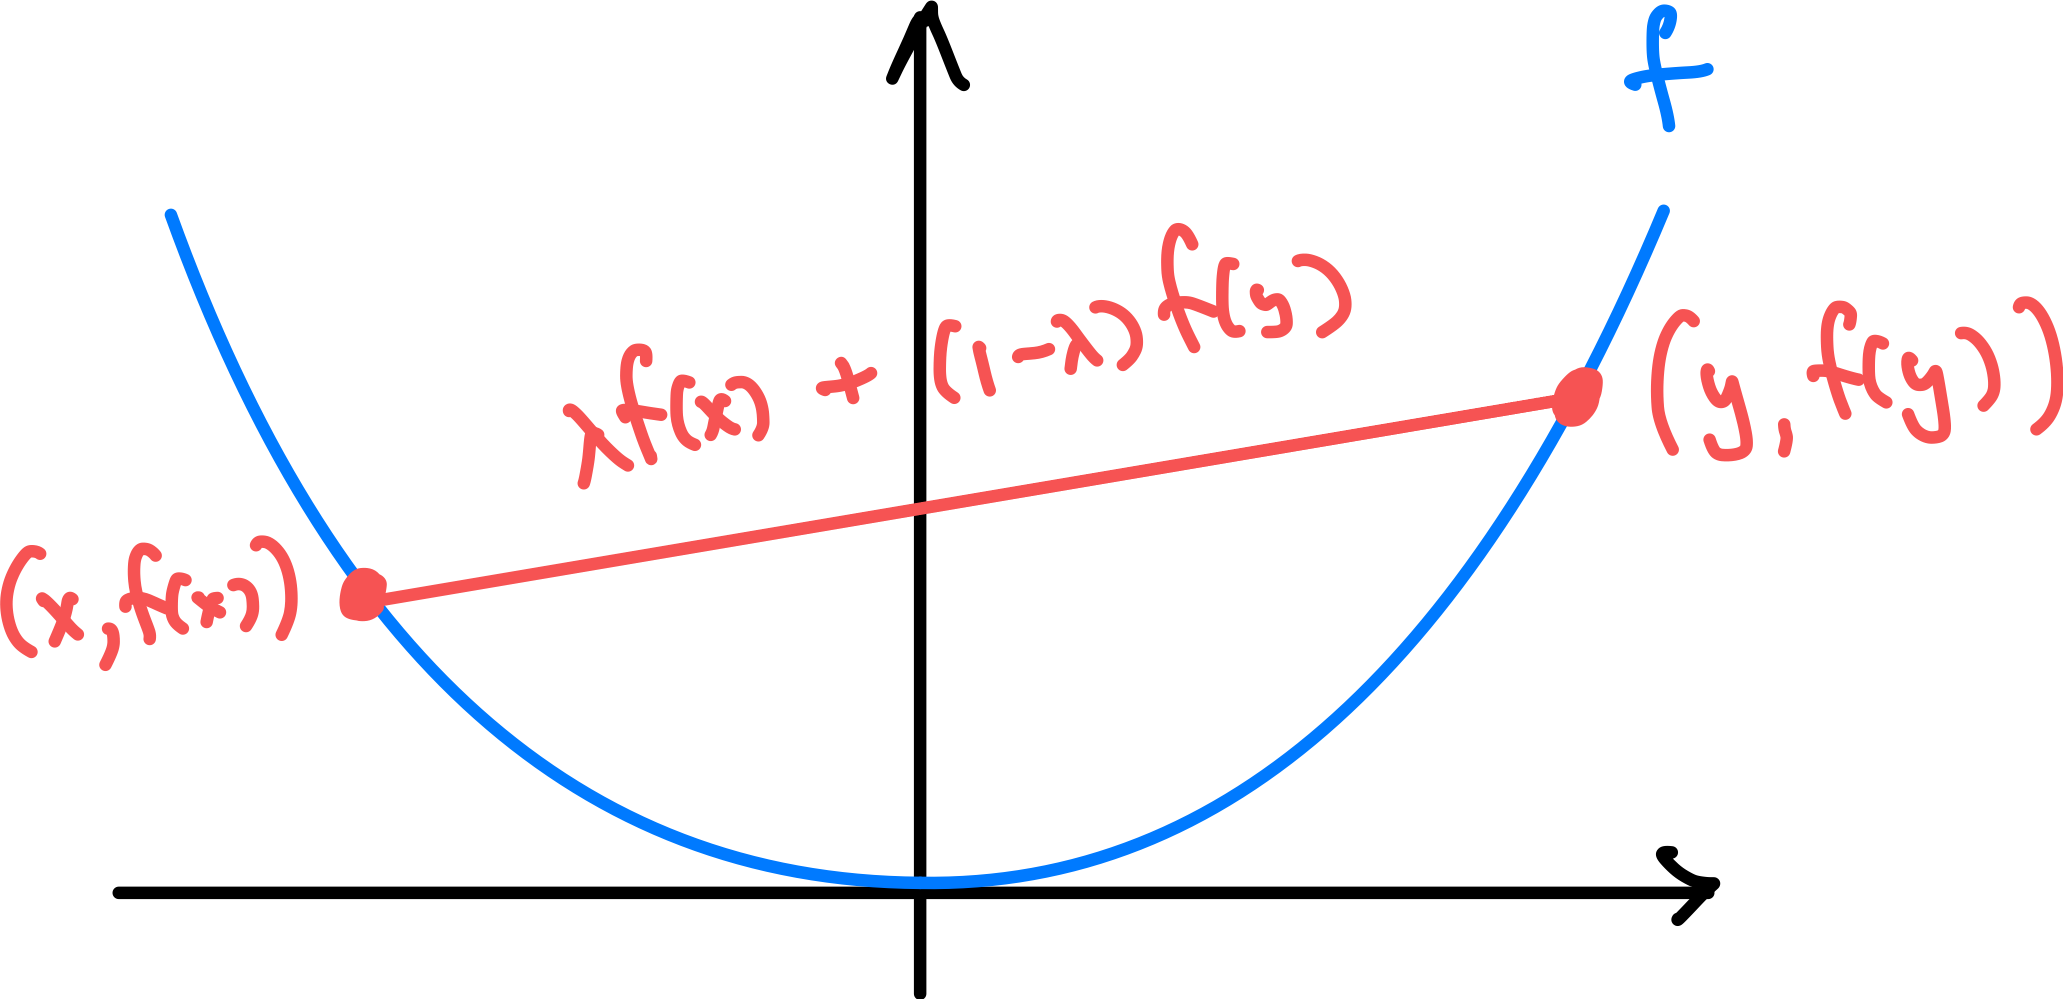
\includegraphics[width=0.5\textwidth]{Figs/convex_function.png}
    \caption{Convex function}
\end{figure}

\begin{theorem} (Characterization via epigraph): A function $f : S \to \mathbb{R}$ is convex if and only if its epigraph $\{(x,t) \in S \times \mathbb{R} : f(x) \leq t\}$ is a convex set.
\end{theorem}

\begin{figure}[H]
    \centering
    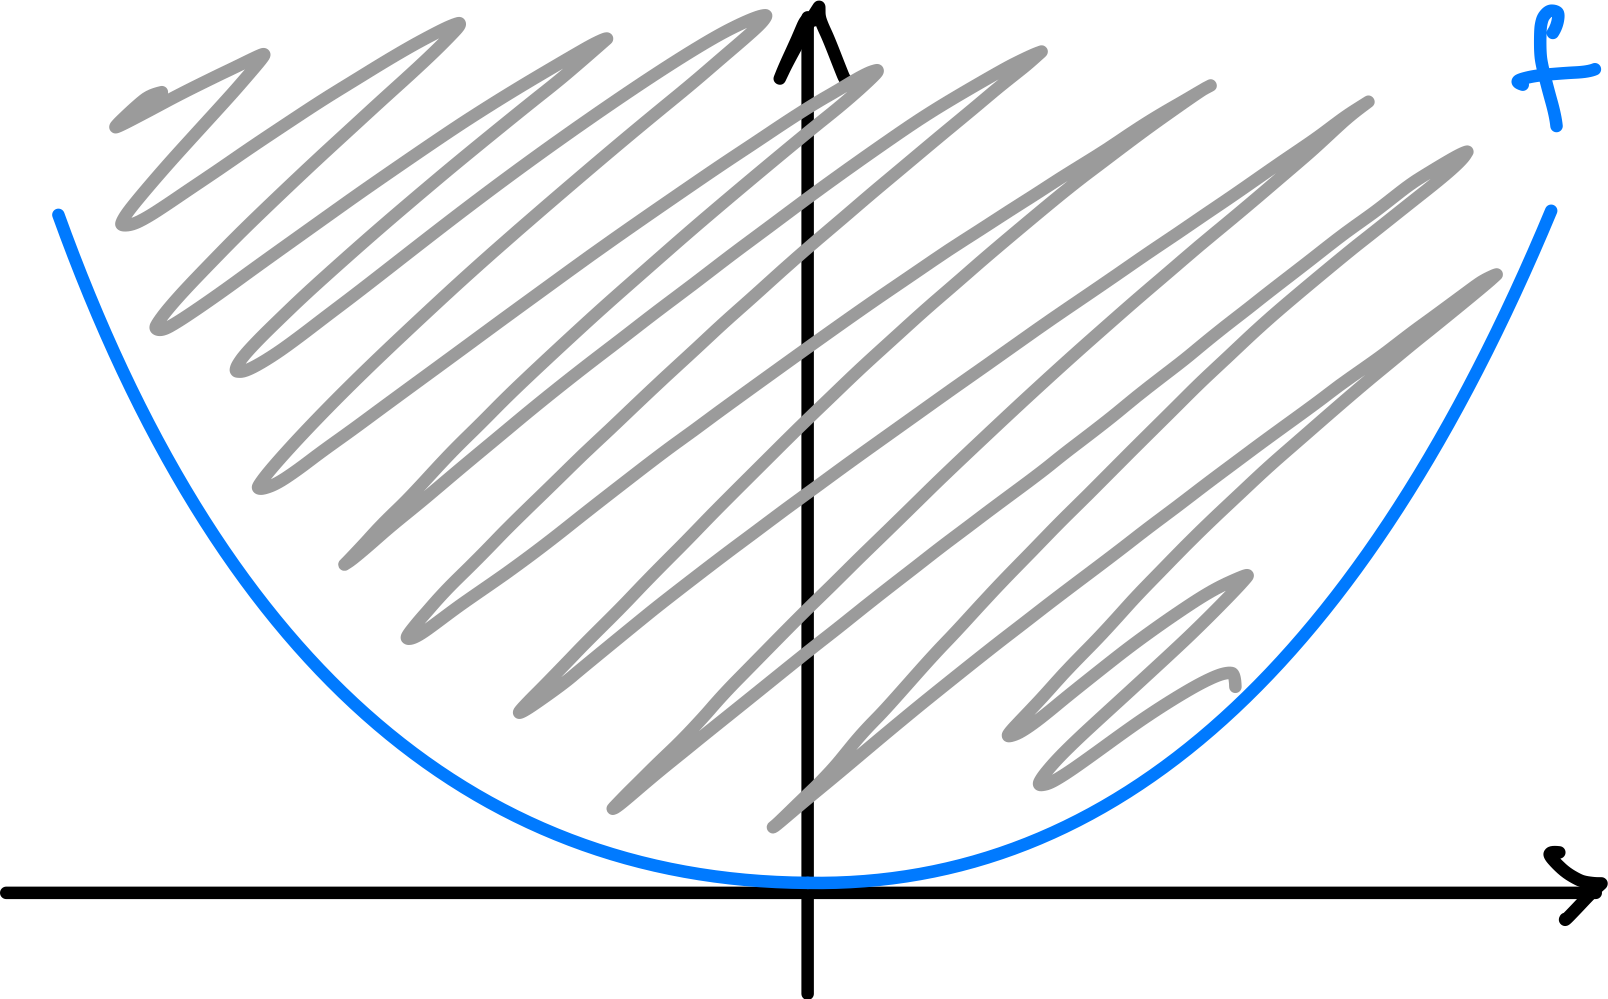
\includegraphics[width=0.3\textwidth]{Figs/epigraph_of_convex_function.png}
    \caption{Epigraph of a convex function}
\end{figure}


\begin{claim} (Convexity of sublevel sets): If $f : S \to \mathbb{R}$ is convex, then the sublevel set $S_t = \{ x \in S : f(x) \leq t\}$ is convex for any $t \in \mathbb{R}$.
\end{claim}

% * * * * * * * * * * * * * * * * * * * * * * * * * * * * * * * * * * * * * * * * * * * * * * * *
% * * * * * * * * * * * * * * * * * * * * * * * * * * * * * * * * * * * * * * * * * * * * * * * *
% * * * * * * * * * * * * * * * * * * * * * * * * * * * * * * * * * * * * * * * * * * * * * * * *
% * * * * * * * * * * * * * * * * * * * * * * * * * * * * * * * * * * * * * * * * * * * * * * * *
% * * * * * * * * * * * * * * * * * * * * * * * * * * * * * * * * * * * * * * * * * * * * * * * *
% * * * * * * * * * * * * * * * * * * * * * * * * * * * * * * * * * * * * * * * * * * * * * * * *
% * * * * * * * * * * * * * * * * * * * * * * * * * * * * * * * * * * * * * * * * * * * * * * * *
% * * * * * * * * * * * * * * * * * * * * * * * * * * * * * * * * * * * * * * * * * * * * * * * *
% * * * * * * * * * * * * * * * * * * * * * * * * * * * * * * * * * * * * * * * * * * * * * * * *
% * * * * * * * * * * * * * * * * * * * * * * * * * * * * * * * * * * * * * * * * * * * * * * * *
% * * * * * * * * * * * * * * * * * * * * * * * * * * * * * * * * * * * * * * * * * * * * * * * *
% * * * * * * * * * * * * * * * * * * * * * * * * * * * * * * * * * * * * * * * * * * * * * * * *
% * * * * * * * * * * * * * * * * * * * * * * * * * * * * * * * * * * * * * * * * * * * * * * * *
% * * * * * * * * * * * * * * * * * * * * * * * * * * * * * * * * * * * * * * * * * * * * * * * *
% * * * * * * * * * * * * * * * * * * * * * * * * * * * * * * * * * * * * * * * * * * * * * * * *
% * * * * * * * * * * * * * * * * * * * * * * * * * * * * * * * * * * * * * * * * * * * * * * * *
% * * * * * * * * * * * * * * * * * * * * * * * * * * * * * * * * * * * * * * * * * * * * * * * *
% * * * * * * * * * * * * * * * * * * * * * * * * * * * * * * * * * * * * * * * * * * * * * * * *
% * * * * * * * * * * * * * * * * * * * * * * * * * * * * * * * * * * * * * * * * * * * * * * * *
% * * * * * * * * * * * * * * * * * * * * * * * * * * * * * * * * * * * * * * * * * * * * * * * *
% * * * * * * * * * * * * * * * * * * * * * * * * * * * * * * * * * * * * * * * * * * * * * * * *

\chapter{Inequalities and Characterizations}

\begin{theorem}(Jensen's inequality): If $f$ is a convex function, then for any $x_1, x_2, \ldots, x_n \in S$ and any non-negative weights $\alpha_i$ such that $\sum_{i=1}^n \alpha_i = 1$,
\[ f\left(\sum_{i=1}^n \alpha_i x_i\right) \leq \sum_{i=1}^n \alpha_i f(x_i). \]
\end{theorem}


\begin{theorem}(First-order characterization, aka “the gradient inequality”): If $f$ is a differentiable convex function on an open set $S$, then for all $x, y \in S$,
\[ f(y) \geq f(x) + \nabla f(x)^\top (y - x). \]
\end{theorem}

\begin{figure}[H]
    \centering
    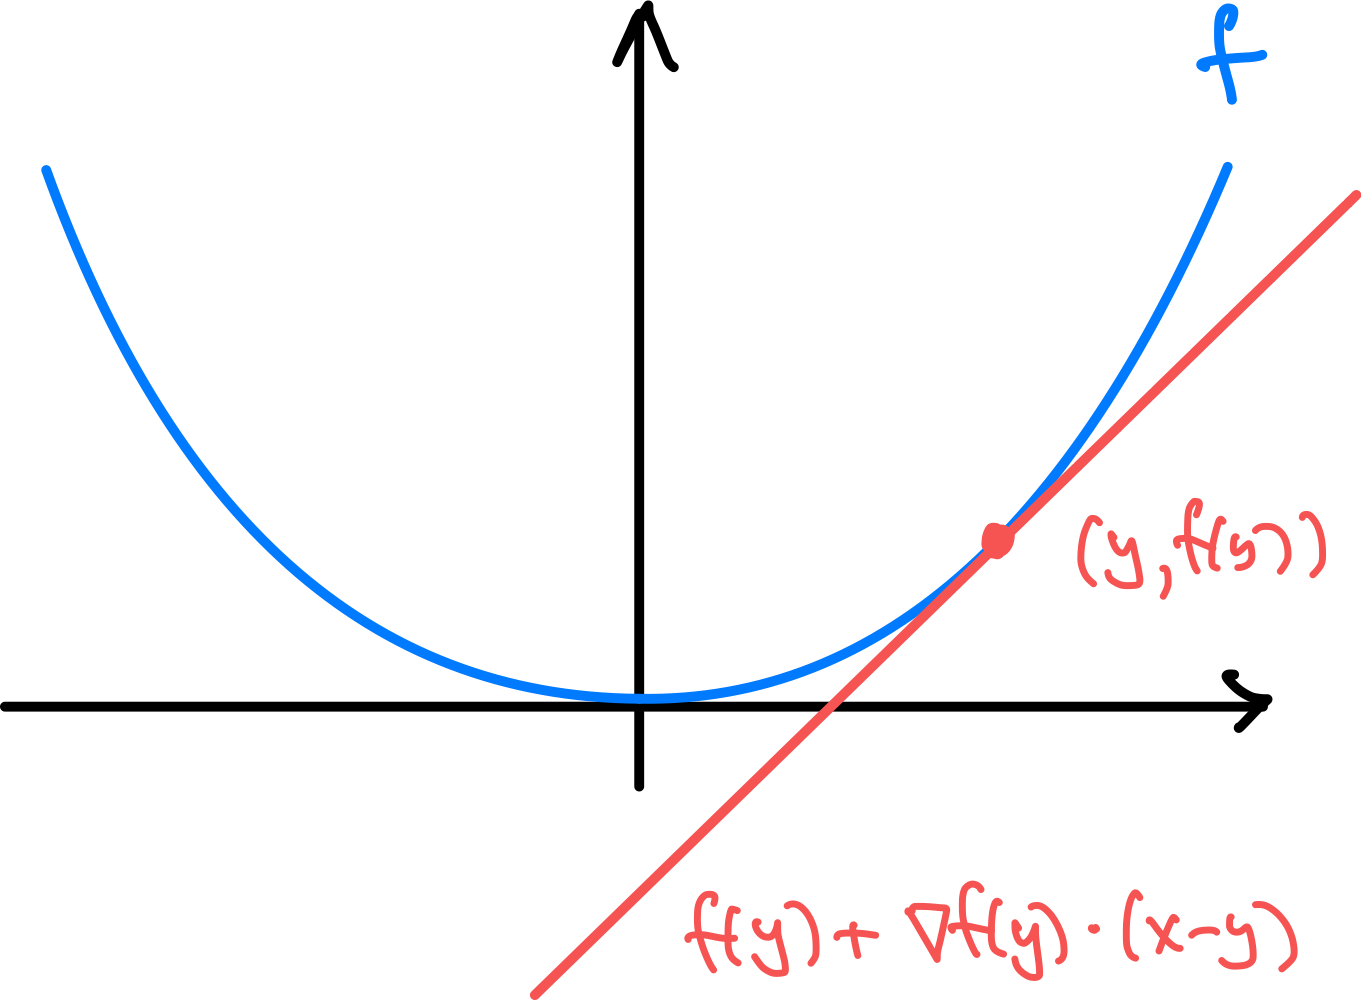
\includegraphics[width=0.3\textwidth]{Figs/first_order_characterization_of_convexity.png}
    \caption{First-order characterization of convexity}
\end{figure}

\begin{definition}{Bergman divergence (distance)} \\
The Bergman divergence between two points $x, y \in \mathbb{R}^n$ is defined as
\begin{equation}
    D_f(x,y) = f(x) - f(y) - \nabla f(y)^\top (x-y)
\end{equation}
\end{definition}


\begin{theorem} (Jensen’s inequality, generalized for expectation): If $f$ is a convex function and $X$ is a random variable over $S$, then
\[ f(\mathbb{E}[X]) \leq \mathbb{E}[f(X)]. \]
\end{theorem}


\begin{theorem} (Second-order characterization of convexity): A twice differentiable function $f$ is convex on an open set $S$ if and only if the Hessian matrix of $f$ is positive semidefinite at every point in $S$.
\end{theorem}

% * * * * * * * * * * * * * * * * * * * * * * * * * * * * * * * * * * * * * * * * * * * * * * * *
% * * * * * * * * * * * * * * * * * * * * * * * * * * * * * * * * * * * * * * * * * * * * * * * *
% * * * * * * * * * * * * * * * * * * * * * * * * * * * * * * * * * * * * * * * * * * * * * * * *
% * * * * * * * * * * * * * * * * * * * * * * * * * * * * * * * * * * * * * * * * * * * * * * * *
% * * * * * * * * * * * * * * * * * * * * * * * * * * * * * * * * * * * * * * * * * * * * * * * *
% * * * * * * * * * * * * * * * * * * * * * * * * * * * * * * * * * * * * * * * * * * * * * * * *
% * * * * * * * * * * * * * * * * * * * * * * * * * * * * * * * * * * * * * * * * * * * * * * * *
% * * * * * * * * * * * * * * * * * * * * * * * * * * * * * * * * * * * * * * * * * * * * * * * *
% * * * * * * * * * * * * * * * * * * * * * * * * * * * * * * * * * * * * * * * * * * * * * * * *
% * * * * * * * * * * * * * * * * * * * * * * * * * * * * * * * * * * * * * * * * * * * * * * * *
% * * * * * * * * * * * * * * * * * * * * * * * * * * * * * * * * * * * * * * * * * * * * * * * *
% * * * * * * * * * * * * * * * * * * * * * * * * * * * * * * * * * * * * * * * * * * * * * * * *
% * * * * * * * * * * * * * * * * * * * * * * * * * * * * * * * * * * * * * * * * * * * * * * * *
% * * * * * * * * * * * * * * * * * * * * * * * * * * * * * * * * * * * * * * * * * * * * * * * *
% * * * * * * * * * * * * * * * * * * * * * * * * * * * * * * * * * * * * * * * * * * * * * * * *
% * * * * * * * * * * * * * * * * * * * * * * * * * * * * * * * * * * * * * * * * * * * * * * * *
% * * * * * * * * * * * * * * * * * * * * * * * * * * * * * * * * * * * * * * * * * * * * * * * *
% * * * * * * * * * * * * * * * * * * * * * * * * * * * * * * * * * * * * * * * * * * * * * * * *
% * * * * * * * * * * * * * * * * * * * * * * * * * * * * * * * * * * * * * * * * * * * * * * * *
% * * * * * * * * * * * * * * * * * * * * * * * * * * * * * * * * * * * * * * * * * * * * * * * *
% * * * * * * * * * * * * * * * * * * * * * * * * * * * * * * * * * * * * * * * * * * * * * * * *

\chapter{Optimization and Projection}

\begin{definition} (Convex optimization): The problem of minimizing a convex function over a convex set.
\end{definition}

\begin{theorem} (Optimality conditions, unconstrained): If $f$ is convex and differentiable, \\
     $x^*$ is a local minimum of $f$ $\Leftrightarrow$ $x^*$ is a global minimum of $f$ $\Leftrightarrow$  $\nabla f(x^*) = 0$.
\end{theorem}

\begin{theorem} (Optimality conditions, constrained): If $f$ is differentiable and $C$ is a convex set,
     $x^*$ is a local minimum of $f$ on $C$ if and only if $\langle \nabla f(x^*), x - x^* \rangle \geq 0$ for all $x \in C$.
\end{theorem}

\begin{figure}[H]
    \centering
    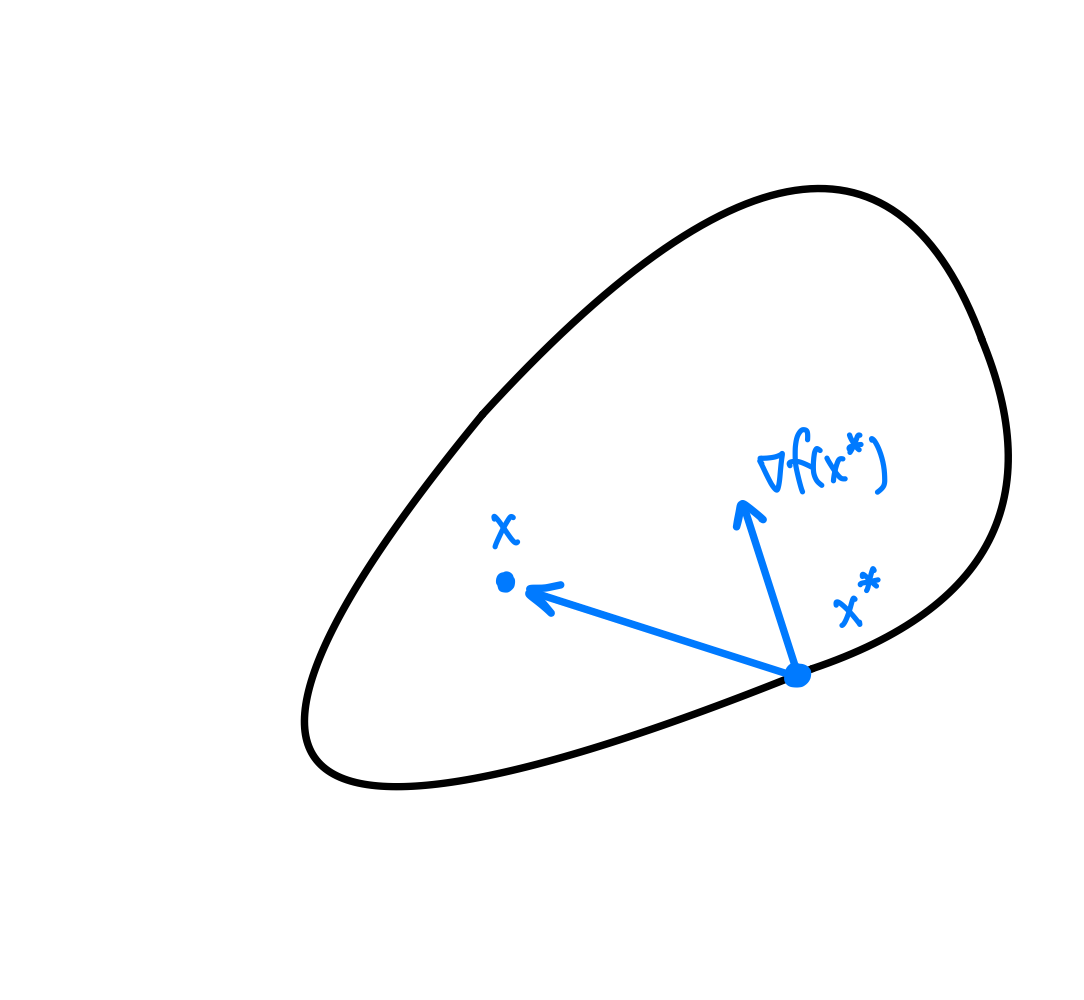
\includegraphics[width=0.5\textwidth]{Figs/optimality_condition_constrained.png}
    \caption{Optimality conditions, constrained}
\end{figure}


\begin{corollary}{Optimality conditions, constrained (alternative)} \\
If $f$ is differentiable and $C$ is a convex set, then $x^*$ is a local minimum of $f$ on $C$ if and only if $-\nabla f(x^*) \in N_C(x^*)$.
\end{corollary}

\begin{definition} (Projection): The projection of a point $x$ onto a convex set $S$ is defined as $\Pi_S(x) = \arg\min_{y \in S} \|y-x\|$.
\end{definition}

\begin{figure}[H]
    \centering
    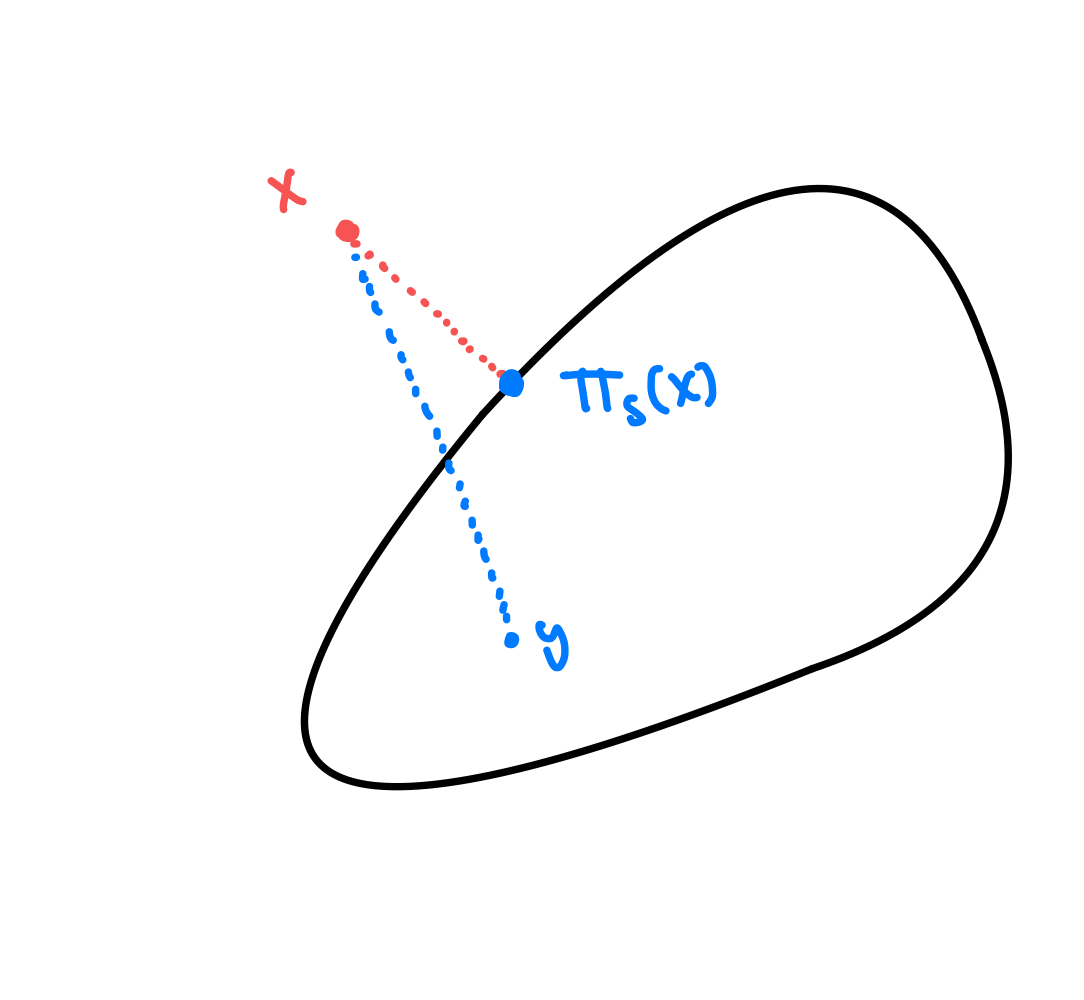
\includegraphics[width=0.3\textwidth]{Figs/projection.png}
    \caption{Projection}
\end{figure}


\begin{theorem} {Generalized cosine theorem} \\
    Let \( S \subseteq \mathbb{R}^d \) be convex and \( x \in \mathbb{R}^d \). Then the projection \( \Pi_S[x] \) is unique and satisfies:
    \begin{equation}
    \| x - \Pi_S[x] \|^2 + \| \Pi_S[x] - y \|^2 \leq \| x - y \|^2, \quad \forall y \in S.
    \end{equation}
    In particular:
    \begin{equation}
    \| \Pi_S[x] - y \| \leq \| x - y \|, \quad \forall y \in S.
    \end{equation}
\end{theorem}


% * * * * * * * * * * * * * * * * * * * * * * * *
% * * * * * * * * * * * * * * * * * * * * * * * *
% * * * * * * * * * * * * * * * * * * * * * * * *
% * * * * * * * * * * * * * * * * * * * * * * * *
% * * * * * * * * * * * * * * * * * * * * * * * *
% * * * * * * * * * * * * * * * * * * * * * * * *
% * * * * * * * * * * * * * * * * * * * * * * * *

% * * * * * * * * * * * * * * * * * * * * * * * * * * * * * * * * * * * * * * * * * * * * * * * *
% * * * * * * * * * * * * * * * * * * * * * * * * * * * * * * * * * * * * * * * * * * * * * * * *
% * * * * * * * * * * * * * * * * * * * * * * * * * * * * * * * * * * * * * * * * * * * * * * * *
% * * * * * * * * * * * * * * * * * * * * * * * * * * * * * * * * * * * * * * * * * * * * * * * *
% * * * * * * * * * * * * * * * * * * * * * * * * * * * * * * * * * * * * * * * * * * * * * * * *
% * * * * * * * * * * * * * * * * * * * * * * * * * * * * * * * * * * * * * * * * * * * * * * * *
% * * * * * * * * * * * * * * * * * * * * * * * * * * * * * * * * * * * * * * * * * * * * * * * *
% * * * * * * * * * * * * * * * * * * * * * * * * * * * * * * * * * * * * * * * * * * * * * * * *
% * * * * * * * * * * * * * * * * * * * * * * * * * * * * * * * * * * * * * * * * * * * * * * * *
% * * * * * * * * * * * * * * * * * * * * * * * * * * * * * * * * * * * * * * * * * * * * * * * *
% * * * * * * * * * * * * * * * * * * * * * * * * * * * * * * * * * * * * * * * * * * * * * * * *
% * * * * * * * * * * * * * * * * * * * * * * * * * * * * * * * * * * * * * * * * * * * * * * * *
% * * * * * * * * * * * * * * * * * * * * * * * * * * * * * * * * * * * * * * * * * * * * * * * *
% * * * * * * * * * * * * * * * * * * * * * * * * * * * * * * * * * * * * * * * * * * * * * * * *
% * * * * * * * * * * * * * * * * * * * * * * * * * * * * * * * * * * * * * * * * * * * * * * * *
% * * * * * * * * * * * * * * * * * * * * * * * * * * * * * * * * * * * * * * * * * * * * * * * *
% * * * * * * * * * * * * * * * * * * * * * * * * * * * * * * * * * * * * * * * * * * * * * * * *
% * * * * * * * * * * * * * * * * * * * * * * * * * * * * * * * * * * * * * * * * * * * * * * * *
% * * * * * * * * * * * * * * * * * * * * * * * * * * * * * * * * * * * * * * * * * * * * * * * *
% * * * * * * * * * * * * * * * * * * * * * * * * * * * * * * * * * * * * * * * * * * * * * * * *
% * * * * * * * * * * * * * * * * * * * * * * * * * * * * * * * * * * * * * * * * * * * * * * * *

\chapter{Smooth Optimization}
\todo[inline]{Add the definitions and remove unrelated content.}

\begin{definition}{L - Lipschitz continuous} \\
A function $f: S \rightarrow \mathbb{R}$ is L-Lipschitz continuous if for all $x, y \in S$,
\begin{equation}
    |f(x) - f(y)| \leq L ||x-y||
\end{equation}    
\end{definition}

\begin{theorem}{Convexity and Lipschitz continuity} \\
If $f$ is convex, differentiable and L-Lipschitz continuous, then $||\nabla f(x)|| \leq L$ for all $x \in S$. 
\end{theorem}

\begin{definition} {Smooth function} \\
    A differentiable function \( f \) is \(\beta\)-smooth over \( S \subseteq \text{dom} f \) if for all \( x, y \in S \):
    \[-\frac{\beta}{2} \|y - x\|^2 \leq f(y) - f(x) - \nabla f(x) \cdot (y - x) \leq \frac{\beta}{2} \|y - x\|^2.\]
\end{definition}


\begin{figure}[H]
    \centering
    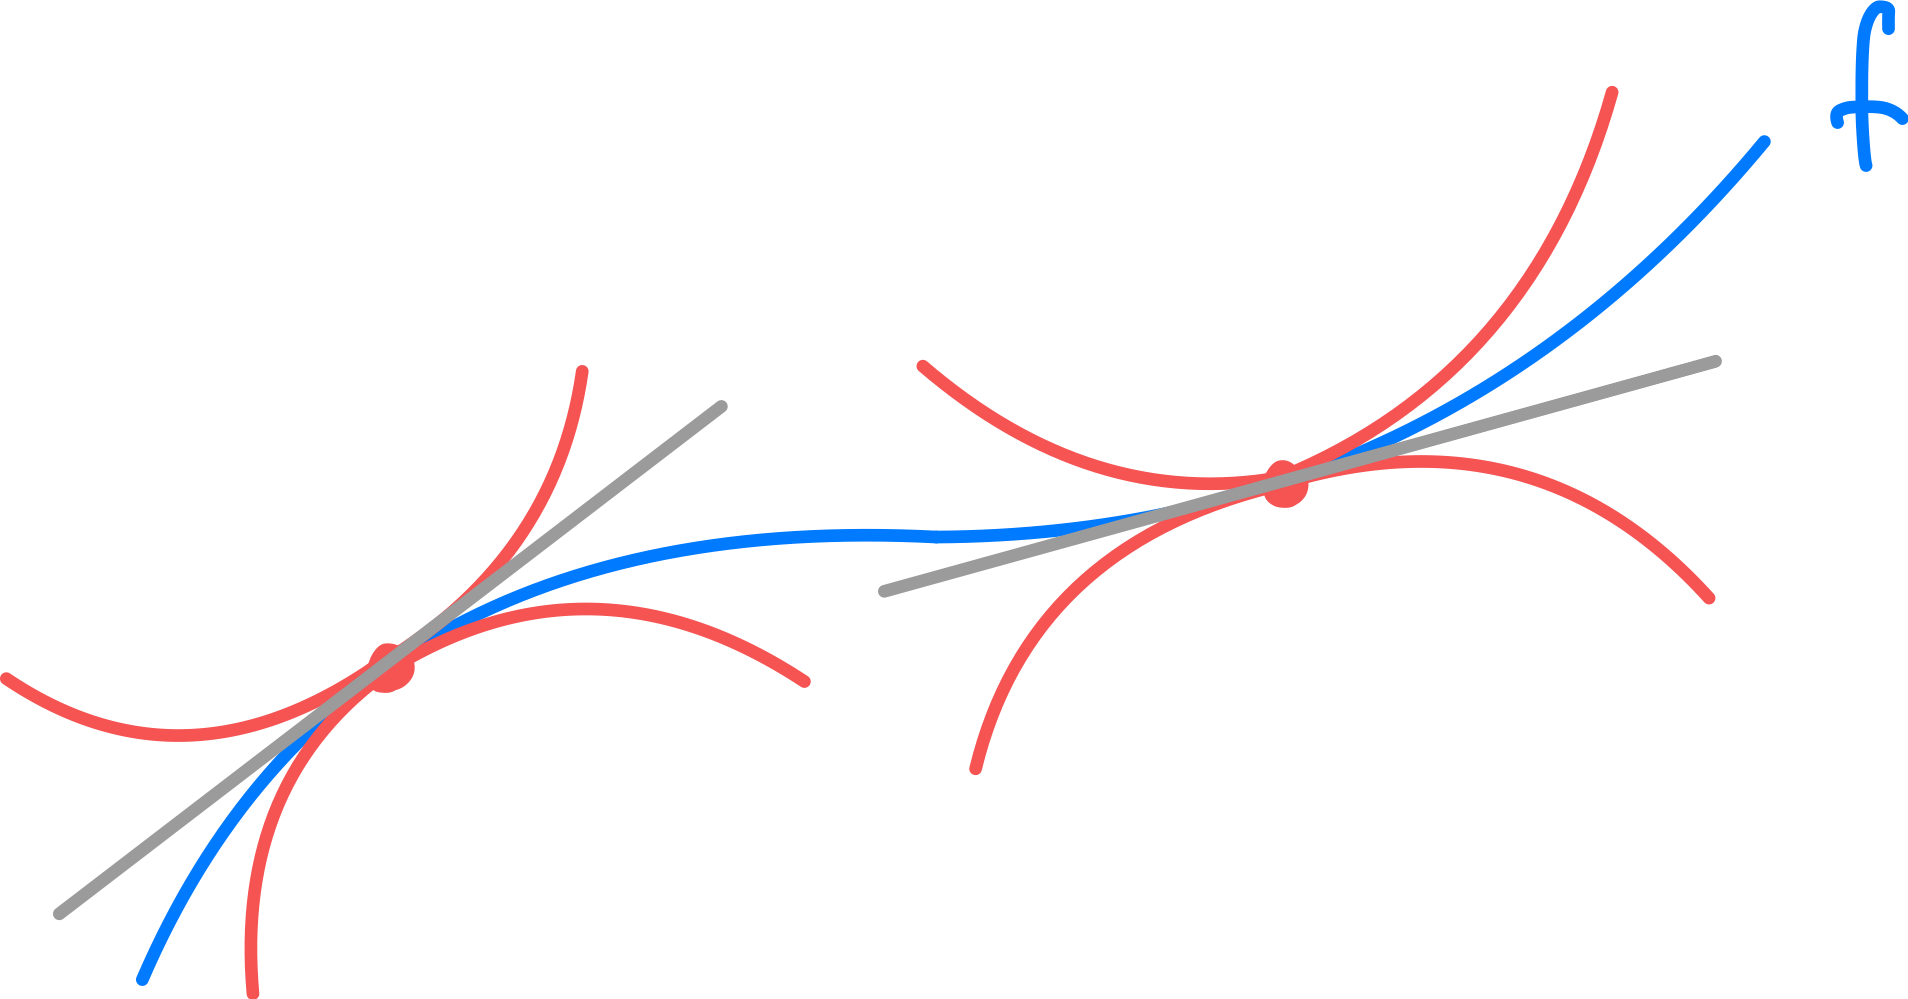
\includegraphics[width=0.7\textwidth]{Figs/beta_smooth_function.png}
    \caption{Smooth function}
\end{figure}


\begin{theorem} {Lipschitz gradient interpretation } \\
Let \( f \) be differentiable and let \( S \subseteq \text{dom} f \) be convex and closed. Suppose that
\[\|\nabla f(x) - \nabla f(y)\| \leq \beta \|x - y\|, \quad \forall x, y \in S.\]
Then \( f \) is \(\beta\)-smooth over \( S \).
\end{theorem}

\begin{theorem} {Second-order characterization of smoothness} \\
Let \( f \) be \( C^2 \) and let \( S \subseteq \text{dom} f \) be convex and closed. Then \( f \) is \(\beta\)-smooth over \( S \) if and only if
\[-\beta I \preceq \nabla^2 f(x) \preceq \beta I, \quad \forall x \in S.\]
\end{theorem}


\begin {lemma} {The Descent Lemma} \\
Let \( f : \mathbb{R}^d \rightarrow \mathbb{R} \) be \(\beta\)-smooth, and let \( x \in \mathbb{R}^d \).
\end{lemma}

\begin{itemize}
    \item For \( \eta \leq \frac{1}{\beta} \), \( x^{+} = x - \eta \nabla f(x) \), we have
    \[ f(x^{+}) - f(x) \leq -\frac{\eta}{2} \|\nabla f(x)\|^2. \]
    \item For \( x^{*} \in \text{arg\,min}_x f(x) \), we have
    \[ \frac{1}{2\beta} \|\nabla f(x)\|^2 \leq f(x) - f(x^{*}). \]
\end{itemize}

\textbf{Basic Facts}:
\begin{itemize}
    \item An affine function \( f : \mathbb{R}^d \rightarrow \mathbb{R}, f(x) = a^\top x + b \), is 0-smooth.
    \item A quadratic function \( f : \mathbb{R}^d \rightarrow \mathbb{R}, f(x) = \frac{1}{2} x^\top A x + b^\top x + c \), is \( \lambda_{\text{max}}(A) \)-smooth.
    \item A linear combination of smooth functions is smooth with an appropriate parameter.
    \item A convex combination of \(\beta\)-smooth functions is \(\beta\)-smooth.
\end{itemize}

\section{"Proximal" view of smooth optimization}

Our initial motivation for introducing smoothness was for ensuring that the gradient $\nabla f(x_t)$ 
(used in the optimization step) is indeed a faithful representative of the local behavior of the objective $f$ around $x_t$.

We formalized this by a requirement that the linear approximation of $f$ at $x_t$ is not too far from $f$ close to $x_t$: 
\[
f(x) \leq f(x_t) + \nabla f(x_t) \cdot (x - x_t) + \frac{\beta}{2} \|x - x_t\|^2.
\]
(We ignore the symmetric lower bound since we are still focusing on convex $f$.)

Revisiting this approach, a tempting idea is to use this approximation of $f$ for algorithm design: since it is easy to minimize a quadratic, we can try to construct $x_{t+1}$ by minimizing the RHS of the upper bound above.

\begin{figure}[H]
    \centering
    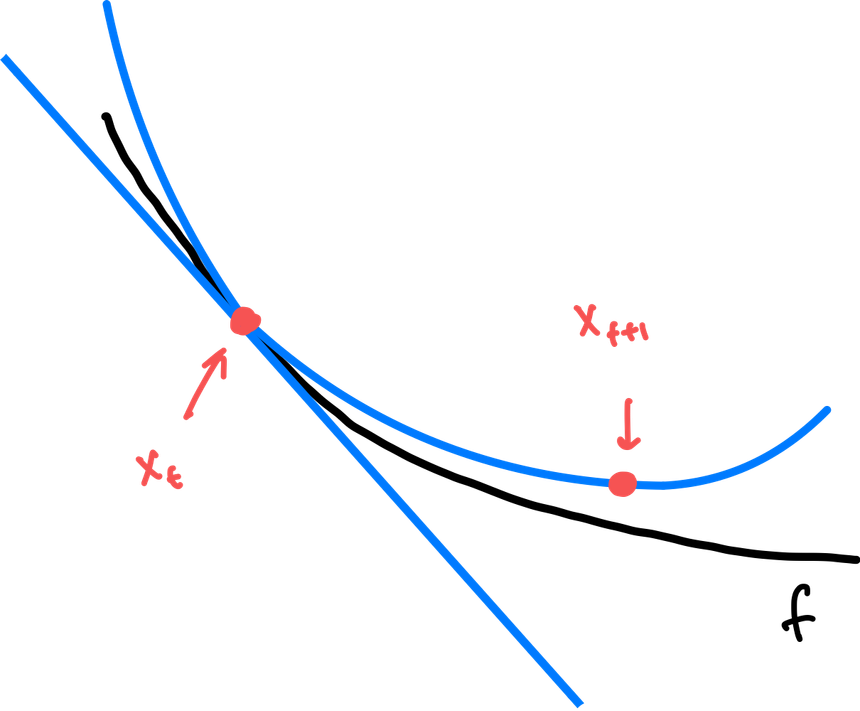
\includegraphics[width=0.4\textwidth]{Figs/proximal_view_of_smooth_optimization.png}
    \caption{Proximal view of smooth optimization}
\end{figure}

To solve this, let's take the gradient with respect to \( y \) and equate to zero:
\[
\nabla f(x_t) + \beta (x_{t+1} - x_t) = 0 \Rightarrow x_{t+1} = x_t - \frac{1}{\beta} \nabla f(x_t).
\]
This precisely gives gradient descent with \( \eta = \frac{1}{\beta} \)!

\begin{remark*}{\textbf{Gradient Descent as Proximal Operator}} \\
    Given a convex and \(\beta\)-smooth \( f \colon \mathbb{R}^d \rightarrow \mathbb{R} \) and starting from \( x_1 \in \mathbb{R}^d \), compute for \( t = 1, 2, \dots \):
    \[
    x_{t+1} = \arg\min_{x \in \mathbb{R}^d} \left\{ f(x_t) + \nabla f(x_t) \cdot (x - x_t) + \frac{\beta}{2} \| x - x_t \|^2 \right\}.
     \]
\end{remark*}

\medbreak

This motivates the following definition, central to convex optimization:

\begin{definition}{\textbf{Proximal operator (``prox'')}} \\
    The proximal operator associated with a convex function \( h \colon \mathbb{R}^d \rightarrow \mathbb{R} \) is:
    \[
    \text{prox}_{h,\eta}(x) = \arg\min_{y \in \mathbb{R}^d} \left\{ h(y) + \frac{1}{2\eta} \| y - x \|^2 \right\}
    \]
\end{definition}

Thus, a step of (unconstrained) gradient descent can be viewed as a proximal operator
\[
x_{t+1} = \text{prox}_{h_t, 1/\beta}(x_t),
\]
applied to a linearization \( h_t \) of \( f \) at \( x_t \):
\[
h_t(x) = f(x_t) + \nabla f(x_t) \cdot (x - x_t).
\]

A similar equivalence also holds in the constrained case.

\subsection{Proximal point and implicit updates}

What happens if we apply the proximal operator without linearizations?

Given a convex function \( f \colon \mathbb{R}^d \to \mathbb{R} \) and step size \( \eta > 0 \), consider:
\[
x_{t+1} = \text{prox}_{f,\eta}(x_t), \quad t = 1, 2, \dots
\]
\begin{itemize}
  \item Note that computing the proximal mapping now becomes a convex optimization problem that needs to be solved at each step...
  \item In other words: this is not a ``real'' algorithm, in the sense that it is not directly implementable in the standard gradient oracle model.
\end{itemize}

Let us compute the proximal operator by solving the minimization in the definition:
\[
x_{t+1} = \text{prox}_{f,\eta}(x_t) = \arg \min_{y \in \mathbb{R}^d} \left\{ f(y) + \frac{1}{2\eta} \| y - x_t \|^2 \right\}
\]
\[
\iff \nabla f(x_{t+1}) + \frac{1}{\eta}(x_{t+1} - x_t) = 0
\]
\[
\iff x_{t+1} = x_t - \eta \nabla f(x_{t+1}).
\]
\begin{itemize}
  \item We see that \( x_{t+1} \) is defined via a gradient descent step, but with the gradient evaluated at \( x_{t+1} \) rather than at \( x_t \)!
  \item This is called an ``implicit update'' in the machine learning literature, since \( x_{t+1} \) is defined via an implicit equation.
\end{itemize}

Say that we can actually compute proximal mappings with respect to \( f \). How powerful is this?

\begin{theorem}{\textbf{Convergence of proximal point updates}} \\
    Let \( f \colon \mathbb{R}^d \to \mathbb{R} \) be convex. Then for proximal updates with respect to \( f \) with any \( \eta > 0 \) we have for any \( x^* \in \mathbb{R}^d \):
    \[
    f(\hat{x}_{T+1}) - f(x^*) \leq \frac{\| x_1 - x^* \|^2}{2\eta T},
    \]
    where \( \hat{x}_{T+1} \) is either the averaged \( \bar{x}_{T+1} = \frac{1}{T} \sum_{t=1}^T x_{t+1} \) or the final \( x_{T+1} \).
\end{theorem}

\begin{itemize}  
  \item Note the generality: we only assume \( f \) is convex. No smoothness assumptions --- \( f \) need not be even Lipschitz!
  \item The result also holds for any positive step size --- it can be as large as we want, making convergence as fast as we want. Why does this make sense? (E.g., what happens when \( \eta \to \infty \)?)
  \item Again, recall that this is not a ``real'' algorithm: we are asked to solve a ``full'' optimization problem at each step to make this work... However, the analysis of this hypothetical algorithm already contains most of the ideas of actually-useful methods.
\end{itemize}


\begin{proof}
    Apply the fundamental inequality with \( g_t = \nabla f(x_{t+1}) \); we obtain
    \[
    \sum_{t=1}^{T} \nabla f(x_{t+1}) \cdot (x_t - x^*) \leq \frac{\| x_1 - x^* \|^2}{2\eta} + \frac{\eta}{2} \sum_{t=1}^{T} \| \nabla f(x_{t+1}) \|^2.
    \]
    
    Observe that, by convexity,
    \begin{align*}
    \nabla f(x_{t+1}) \cdot (x_t - x^*) &= \nabla f(x_{t+1}) \cdot (x_{t+1} - x^*) + \nabla f(x_{t+1}) \cdot (x_t - x_{t+1}) \\
    &= \nabla f(x_{t+1}) \cdot (x_{t+1} - x^*) + \nabla f(x_{t+1}) \cdot (\eta \nabla f(x_{t+1})) \\
    &\geq f(x_{t+1}) - f(x^*) + \eta \| \nabla f(x_{t+1}) \|^2
    \end{align*}
    
    Together we get
    \[
    \sum_{t=1}^{T} f(x_{t+1}) - f(x^*) \leq \frac{\| x_1 - x^* \|^2}{2\eta} - \frac{\eta}{2} \sum_{t=1}^{T} \| \nabla f(x_{t+1}) \|^2.
    \]
    
    By simply discarding the negative term on the RHS and dividing by \( T \), we obtain
    \[
    \frac{1}{T} \sum_{t=1}^{T} f(x_{t+1}) - f(x^*) \leq \frac{\| x_1 - x^* \|^2}{2\eta T}.
    \]
    
    This implies the rate for the average \( \bar{x}_{T+1} \) via Jensen's, and for the final iterate \( x_{T+1} \) by the monotonicity of the updates. (To see that \( f(x_{t+1}) \leq f(x_t) \) for all \( t \), simply let \( y = x_t \) in the definition of prox...)
\end{proof}


\subsection{Proximal Point method}

Proximal point iterations are only useful when we can compute the internal minimization at each step efficiently. We have seen that:
\begin{itemize}
  \item proximal point iterations with linearizations give rise to plain old gradient descent, which converges quickly only for smooth objectives;
  \item proximal point iterations with the original objective \( f \) always converge quickly but require solving a full optimization problem at each step.
\end{itemize}

Is there a finer balance between the two?

The idea of proximal point iterations can indeed be generalized much further, and has multiple applications in optimization. We will discuss the following general version:

\begin{algorithm}[H]
    \caption{Proximal Point method} \label{alg:proximal_point_method}
    Given a function \( f \colon \mathbb{R}^d \to \mathbb{R} \) and step size \( \eta > 0 \), compute:
    \[ x_{t+1} = \text{prox}_{h_t,\eta}(x_t), \quad t = 1, 2, \ldots \]
    where \( h_t \colon \mathbb{R}^d \to \mathbb{R} \) are convex functions such that
    \[ \forall x \in \mathbb{R}^d \colon h_t(x) \leq f(x) \leq h_t(x) + \frac{\beta}{2} \| x - x_t \|^2. \]    
\end{algorithm}

\begin{itemize}
    \item \( h_t \) are “tight lower approximations” of \( f \): like linear approximations for \( \beta \)-smooth and convex functions, but could be much more general.
    \item In particular, for \( x = x_t \) this implies \( h_t(x_t) = f(x_t) \); namely, the approximation \( h_t \) coincides with \( f \) at \( x = x_t \).
    \item The idea again is that \( h_t \) are “simple enough” so that computing their proximal operator is easy.
    \item Note that \( h_t \) need not be smooth, and not even differentiable — we only assume they are convex.
  \end{itemize}


\begin{figure}[H]
    \centering
    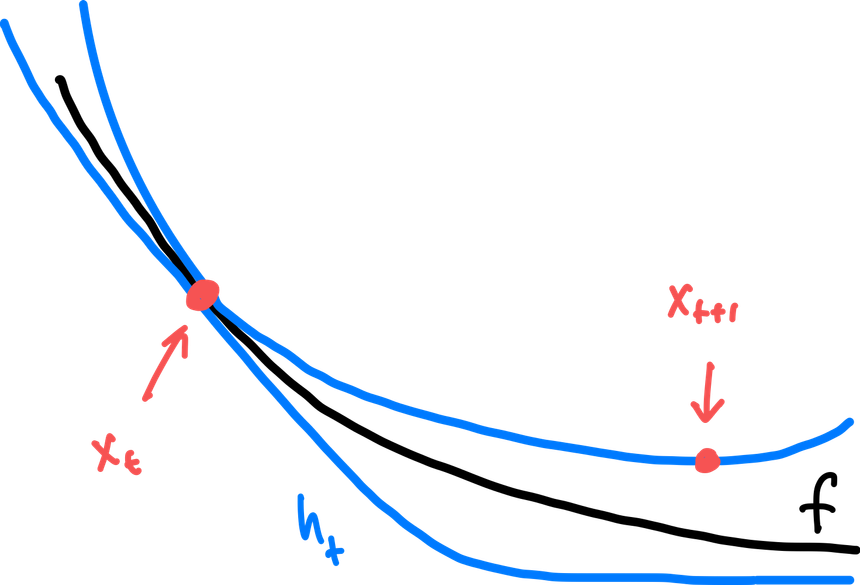
\includegraphics[width=0.5\textwidth]{Figs/proximal_point_method.png}
    \caption{Proximal Point method}
\end{figure}

\subsubsection{Example: the proximal gradient algorithm}

One common example of such a scenario is "composite" optimization problems, of the form:
\[
\min_{x \in \mathbb{R}^d} f(x) = g(x) + h(x),
\]
where:
\begin{itemize}
  \item \( g, h \colon \mathbb{R}^d \rightarrow \mathbb{R} \) are both convex;
  \item \( g \) is \(\beta\)-smooth;
  \item \( h \) is “simple”, in the sense that it has a proximal operator which is easy to compute.
\end{itemize}
Note that \( f \) is not necessarily smooth: we do not assume \( h \) is.

In this case, it makes sense to only “linearize” the smooth \( g \) but keep \( h \) as is. That is, we take approximations of the form:
\[
h_t(x) = g(x_t) + \nabla g(x_t) \cdot (x - x_t) + h(x).
\]

Then, we can compute:
\begin{align*}
    x_{t+1} &= \text{prox}_{h_t,\eta}(x_t) \\
    &= \arg\min_{y \in \mathbb{R}^d} \{ g(x_t) + \nabla g(x_t) \cdot (y - x_t) + h(y) + \frac{1}{2\eta} \| y - x_t \|^2 \} \\
    &= \arg\min_{y \in \mathbb{R}^d} \{ \nabla g(x_t) \cdot y + h(y) + \frac{1}{2\eta} \| y - x_t \|^2 \} \\
    &= \arg\min_{y \in \mathbb{R}^d} \{ h(y) + \frac{1}{2\eta} \| y - (x_t - \eta\nabla g(x_t)) \|^2 \}. 
\end{align*}
That is,
\begin{align*}
    x_{t+1} = \text{prox}_{h,\eta}( x_t - \eta\nabla g(x_t) ) \text{ for } t = 1, 2, \ldots.
\end{align*}

This algorithm is known as the “Proximal gradient algorithm”. We will see shortly that this algorithm enjoys fast convergence as if the objective \( f \) is smooth, even when it is not!


\subsubsection{Example: Back to projected gradient descent}

Consider a special case of composite optimization:
\[
\min_{x \in \mathbb{R}^d} f(x) = g(x) + \delta_S(x),
\]
where \( g \) is a convex and \(\beta\)-smooth function, and \( \delta_S \colon \mathbb{R}^d \to \mathbb{R} \cup \{ \infty \} \) is the indicator function of a convex set \( S \):
\[
\delta_S(x) = 
\begin{cases} 
0 & \text{if } x \in S; \\
\infty & \text{otherwise}.
\end{cases}
\]
Then we can verify that \( \delta_S \) is convex, and the proximal gradient algorithm takes the form:
\[
x_{t+1} = \text{prox}_{\delta_S,\eta}(x_t - \eta\nabla g(x_t)), \quad t = 1, 2, \ldots,
\]
where
\[
\text{prox}_{\delta_S,\eta}(x) = \arg\min_{y \in \mathbb{R}^d} \left\{ \delta_S(y) + \frac{1}{2\eta} \| y - x \|^2 \right\} = \arg\min_{y \in S} \| y - x \|^2 = \Pi_S [x].
\]

(Recall that the proximal gradient algorithm doesn't care whether \( h \) is smooth, or even just differentiable, which is very useful here.)

Therefore, the algorithm takes the form:
\[
x_{t+1} = \Pi_S \left[ x_t - \eta\nabla g(x_t) \right], \quad t = 1, 2, \ldots,
\]
that is: the proximal gradient algorithm in this case is simply projected gradient descent!


\subsubsection{Example: ISTA (Iterative Soft-Thresholding Algorithm)}

Now consider:
\[
\min_x f(x) = \frac{1}{2} \|Ax - b\|^2 + \lambda \|x\|_1.
\]
Here \( g(x) = \frac{1}{2} \|Ax - b\|^2 \) is convex and smooth, and \( h(x) = \lambda \|x\|_1 \) is convex and “simple” in the sense that
\[
\text{prox}_{h,\eta}(x) = \arg\min_y \left\{ \lambda \|y\|_1 + \frac{1}{2\eta} \|y - x\|^2 \right\}
\]
can be computed efficiently in closed-form.

This problem is called LASSO regression, or simply \( L_1 \)-regularized regression, and has many applications in scenarios where sparsity of the solution 
(the number of non-zero coordinates in \( x^* \)) is important.


\subsubsection{Analysis of general proximal point updates}

\begin{algorithm}[H]
    \caption{General Proximal Point method} \label{alg:general_proximal_point_method}
    Given a function \( f \colon \mathbb{R}^d \to \mathbb{R} \) and step size \( \eta > 0 \), compute:
    \[
    x_{t+1} = \text{prox}_{\eta, h_t}(x_t), \quad t = 1, 2, \ldots
    \]
    where \( h_t \colon \mathbb{R}^d \to \mathbb{R} \) are convex functions such that
    \[
    \forall x \in \mathbb{R}^d \colon h_t(x) \leq f(x) \leq h_t(x) + \frac{\beta}{2} \|x - x_t\|^2.
    \]
\end{algorithm}

\medbreak

\begin{theorem}{\textbf{convergence of proximal point updates}} \\
    If \( \eta \leq 1/\beta \), then for any \( x^* \in \mathbb{R}^d \).
    \[
    f(\bar{x}_{T+1}) - f(x^*) \leq \frac{\|x_1 - x^*\|^2}{2\eta T}
    \]
    where \( \bar{x}_{T+1} \) is either the averaged \( \bar{x}_{T+1} = \frac{1}{T} \sum_{t=1}^{T} x_{t+1} \) or the final \( x_{T+1} \).
\end{theorem}

\bigbreak

This implies the same convergence rate for the special cases: proximal gradient algorithm, projected (smooth) gradient descent, ISTA, \ldots


The proof extends ideas we saw before: we express the iteration as an implicit update of the form 
\( x_{t+1} = x_t - \eta \nabla h_t(x_{t+1}) \) and relate \( h_t \) to \( f \ldots \)

\begin{enumerate}
\item Recall that when \( h_t \) are differentiable, we can express an iteration of prox as an implicit update
\[
\forall t = 1, 2, \ldots, \quad x_{t+1} = x_t - \eta \nabla h_t(x_{t+1}).
\]
When \( h_t \) is not differentiable we can write instead \( x_{t+1} = x_t - \eta g_t \) for a suitable subgradient \( g_t \in \partial h_t(x_{t+1}) \).

For simplicity, we will continue assuming \( h_t \) are differentiable; the argument extends directly to the non-differentiable case.

\item Apply the fundamental inequality with \( g_t = \nabla h_t(x_{t+1}) \): for any \( x^* \in \mathbb{R}^d \),
\[
\sum_{t=1}^{T} \nabla h_t(x_{t+1}) \cdot (x_t - x^*) \leq \frac{\|x_1 - x^*\|^2}{2\eta} + \frac{\eta}{2} \sum_{t=1}^{T} \| \nabla h_t(x_{t+1}) \|^2.
\]

\item Let us relate the LHS to the convergence of the algorithm. For any \( x \in \mathbb{R}^d \) we have:
\begin{align*}
\nabla h_t(x_{t+1}) \cdot (x_t - x) &= \nabla h_t(x_{t+1}) \cdot (x_{t+1} - x) + \nabla h_t(x_{t+1}) \cdot (x_t - x_{t+1}) \\
&\geq h_t(x_{t+1}) - h_t(x) + \nabla h_t(x_{t+1}) \cdot \nabla h_t(x_{t+1}) \\
&\geq f(x_{t+1}) - \frac{\beta}{2} \|x_{t+1} - x_t\|^2 - f(x) + \eta \| \nabla h_t(x_{t+1}) \|^2 \\
&= f(x_{t+1}) - f(x) + \left( \eta - \frac{\beta \eta^2}{2} \right) \| \nabla h_t(x_{t+1}) \|^2 \\
&\geq f(x_{t+1}) - f(x) + \frac{\eta}{2} \| \nabla h_t(x_{t+1}) \|^2.
\end{align*}

\item In particular, for \( x = x_t \) we get:
\[
f(x_{t+1}) - f(x_t) \leq -\frac{\eta}{2} \| \nabla h_t(x_{t+1}) \|^2 \leq 0,
\]
that is, the iterations are monotonically descending.

\item Overall, we get
\[
\frac{1}{T} \sum_{t=1}^{T} f(x_{t+1}) - f(x^*) \leq \frac{\| x_1 - x^* \|^2}{2\eta T}.
\]
and the LHS upper bounds both $f(\bar{x}_{T+1}) - f(x^*)$ and $f(x_{T+1}) - f(x^*)$.
\end{enumerate}





% * * * * * * * * * * * * * * * * * * * * * * * * * * * * * * * * * * * * * * * * * * * * * * * *
% * * * * * * * * * * * * * * * * * * * * * * * * * * * * * * * * * * * * * * * * * * * * * * * *
% * * * * * * * * * * * * * * * * * * * * * * * * * * * * * * * * * * * * * * * * * * * * * * * *
% * * * * * * * * * * * * * * * * * * * * * * * * * * * * * * * * * * * * * * * * * * * * * * * *
% * * * * * * * * * * * * * * * * * * * * * * * * * * * * * * * * * * * * * * * * * * * * * * * *
% * * * * * * * * * * * * * * * * * * * * * * * * * * * * * * * * * * * * * * * * * * * * * * * *
% * * * * * * * * * * * * * * * * * * * * * * * * * * * * * * * * * * * * * * * * * * * * * * * *
% * * * * * * * * * * * * * * * * * * * * * * * * * * * * * * * * * * * * * * * * * * * * * * * *
% * * * * * * * * * * * * * * * * * * * * * * * * * * * * * * * * * * * * * * * * * * * * * * * *
% * * * * * * * * * * * * * * * * * * * * * * * * * * * * * * * * * * * * * * * * * * * * * * * *
% * * * * * * * * * * * * * * * * * * * * * * * * * * * * * * * * * * * * * * * * * * * * * * * *
% * * * * * * * * * * * * * * * * * * * * * * * * * * * * * * * * * * * * * * * * * * * * * * * *
% * * * * * * * * * * * * * * * * * * * * * * * * * * * * * * * * * * * * * * * * * * * * * * * *
% * * * * * * * * * * * * * * * * * * * * * * * * * * * * * * * * * * * * * * * * * * * * * * * *
% * * * * * * * * * * * * * * * * * * * * * * * * * * * * * * * * * * * * * * * * * * * * * * * *
% * * * * * * * * * * * * * * * * * * * * * * * * * * * * * * * * * * * * * * * * * * * * * * * *
% * * * * * * * * * * * * * * * * * * * * * * * * * * * * * * * * * * * * * * * * * * * * * * * *
% * * * * * * * * * * * * * * * * * * * * * * * * * * * * * * * * * * * * * * * * * * * * * * * *
% * * * * * * * * * * * * * * * * * * * * * * * * * * * * * * * * * * * * * * * * * * * * * * * *
% * * * * * * * * * * * * * * * * * * * * * * * * * * * * * * * * * * * * * * * * * * * * * * * *
% * * * * * * * * * * * * * * * * * * * * * * * * * * * * * * * * * * * * * * * * * * * * * * * *

\chapter{Strong Convexity}
\todo[inline]{Add the definitions and remove unrelated content.}


\begin{definition} {Strong convexity} \\
A function \( f \) is \(\alpha\)-strongly convex (for \(\alpha \geq 0\)) over a convex and closed set \( S \subseteq \text{dom} f \) if for any \( x \in S \), there exists \( g_x \in \partial f(x) \) such that:
\[
\forall y \in S, \quad f(y) \geq f(x) + g_x \cdot (y - x) + \frac{\alpha}{2} \|y - x\|^2.
\]
In particular, a differentiable \( f \) is \(\alpha\)-strongly convex over \( S \) if for any \( x \in S \),
\[
\forall y \in S, \quad f(y) \geq f(x) + \nabla f(x) \cdot (y - x) + \frac{\alpha}{2} \|y - x\|^2.
\]
\end{definition}

\begin{figure}[H]
    \centering
    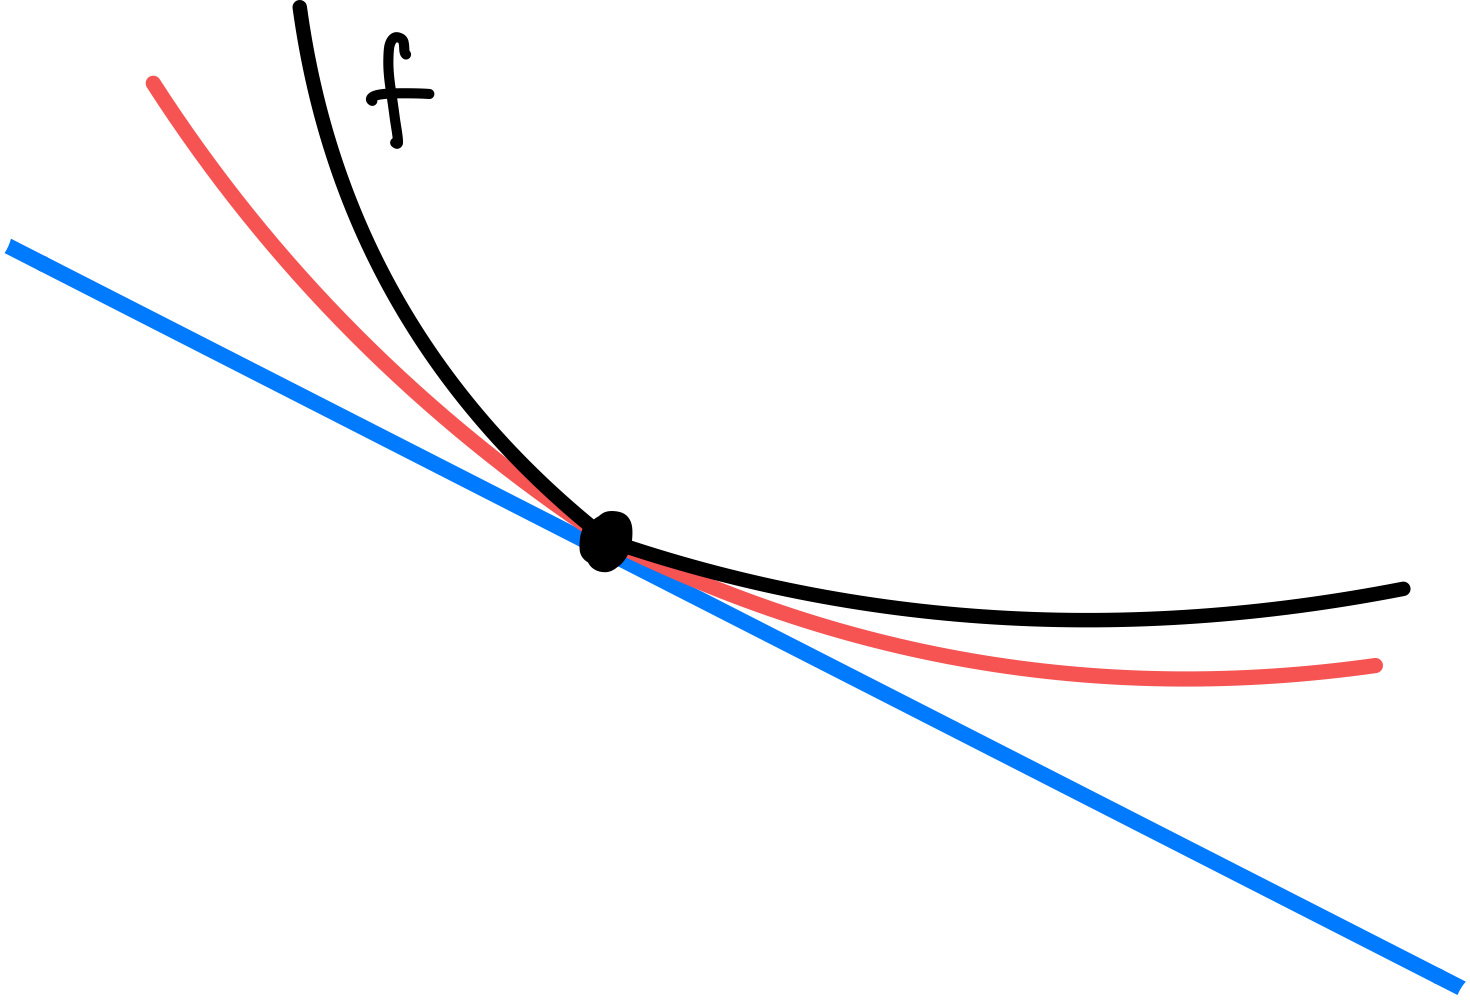
\includegraphics[width=0.5\textwidth]{Figs/strongly_convex.png}
    \caption{Strongly convex function}
\end{figure}

\begin{theorem} { Strong convexity, second-order characterization}\\
Let \( f \) be \( C^2 \) and let \( S \subseteq \text{dom} f \) be convex and closed. Then \( f \) is \(\alpha\)-strongly convex over \( S \) if and only if
\[
\forall x \in S, \quad \nabla^2 f(x) \succeq \alpha I.
\]
\end{theorem}


\begin{theorem} {Usage of strong convexity } \\
If a differentiable \( f \) is \(\alpha\)-strongly convex over a convex and closed \( S \subseteq \text{dom} f \) with a minimum at \( x^* \in S \), then
\[
\forall x \in S, \quad \frac{\alpha}{2} \|x - x^*\|^2 \leq f(x) - f(x^*) \leq \frac{1}{2\alpha} \|\nabla f(x)\|^2.
\]
In particular, the minimum of a strongly convex function is unique.
\end{theorem}




% * * * * * * * * * * * * * * * * * * * * * * * * * * * * * * * * * * * * * * * * * * * * * * * *
% * * * * * * * * * * * * * * * * * * * * * * * * * * * * * * * * * * * * * * * * * * * * * * * *
% * * * * * * * * * * * * * * * * * * * * * * * * * * * * * * * * * * * * * * * * * * * * * * * *
% * * * * * * * * * * * * * * * * * * * * * * * * * * * * * * * * * * * * * * * * * * * * * * * *
% * * * * * * * * * * * * * * * * * * * * * * * * * * * * * * * * * * * * * * * * * * * * * * * *
% * * * * * * * * * * * * * * * * * * * * * * * * * * * * * * * * * * * * * * * * * * * * * * * *
% * * * * * * * * * * * * * * * * * * * * * * * * * * * * * * * * * * * * * * * * * * * * * * * *
% * * * * * * * * * * * * * * * * * * * * * * * * * * * * * * * * * * * * * * * * * * * * * * * *
% * * * * * * * * * * * * * * * * * * * * * * * * * * * * * * * * * * * * * * * * * * * * * * * *
% * * * * * * * * * * * * * * * * * * * * * * * * * * * * * * * * * * * * * * * * * * * * * * * *
% * * * * * * * * * * * * * * * * * * * * * * * * * * * * * * * * * * * * * * * * * * * * * * * *
% * * * * * * * * * * * * * * * * * * * * * * * * * * * * * * * * * * * * * * * * * * * * * * * *
% * * * * * * * * * * * * * * * * * * * * * * * * * * * * * * * * * * * * * * * * * * * * * * * *
% * * * * * * * * * * * * * * * * * * * * * * * * * * * * * * * * * * * * * * * * * * * * * * * *
% * * * * * * * * * * * * * * * * * * * * * * * * * * * * * * * * * * * * * * * * * * * * * * * *
% * * * * * * * * * * * * * * * * * * * * * * * * * * * * * * * * * * * * * * * * * * * * * * * *
% * * * * * * * * * * * * * * * * * * * * * * * * * * * * * * * * * * * * * * * * * * * * * * * *
% * * * * * * * * * * * * * * * * * * * * * * * * * * * * * * * * * * * * * * * * * * * * * * * *
% * * * * * * * * * * * * * * * * * * * * * * * * * * * * * * * * * * * * * * * * * * * * * * * *
% * * * * * * * * * * * * * * * * * * * * * * * * * * * * * * * * * * * * * * * * * * * * * * * *
% * * * * * * * * * * * * * * * * * * * * * * * * * * * * * * * * * * * * * * * * * * * * * * * *

\chapter{Acceleration}

% * * * * * * * * * * * * * * * * * * * * * * * * * * * * * * * * * * * * * * * * * * * * * * * *
% * * * * * * * * * * * * * * * * * * * * * * * * * * * * * * * * * * * * * * * * * * * * * * * *
% * * * * * * * * * * * * * * * * * * * * * * * * * * * * * * * * * * * * * * * * * * * * * * * *
% * * * * * * * * * * * * * * * * * * * * * * * * * * * * * * * * * * * * * * * * * * * * * * * *
% * * * * * * * * * * * * * * * * * * * * * * * * * * * * * * * * * * * * * * * * * * * * * * * *
% * * * * * * * * * * * * * * * * * * * * * * * * * * * * * * * * * * * * * * * * * * * * * * * *
% * * * * * * * * * * * * * * * * * * * * * * * * * * * * * * * * * * * * * * * * * * * * * * * *
% * * * * * * * * * * * * * * * * * * * * * * * * * * * * * * * * * * * * * * * * * * * * * * * *
% * * * * * * * * * * * * * * * * * * * * * * * * * * * * * * * * * * * * * * * * * * * * * * * *
% * * * * * * * * * * * * * * * * * * * * * * * * * * * * * * * * * * * * * * * * * * * * * * * *
% * * * * * * * * * * * * * * * * * * * * * * * * * * * * * * * * * * * * * * * * * * * * * * * *
% * * * * * * * * * * * * * * * * * * * * * * * * * * * * * * * * * * * * * * * * * * * * * * * *
% * * * * * * * * * * * * * * * * * * * * * * * * * * * * * * * * * * * * * * * * * * * * * * * *
% * * * * * * * * * * * * * * * * * * * * * * * * * * * * * * * * * * * * * * * * * * * * * * * *
% * * * * * * * * * * * * * * * * * * * * * * * * * * * * * * * * * * * * * * * * * * * * * * * *
% * * * * * * * * * * * * * * * * * * * * * * * * * * * * * * * * * * * * * * * * * * * * * * * *
% * * * * * * * * * * * * * * * * * * * * * * * * * * * * * * * * * * * * * * * * * * * * * * * *
% * * * * * * * * * * * * * * * * * * * * * * * * * * * * * * * * * * * * * * * * * * * * * * * *
% * * * * * * * * * * * * * * * * * * * * * * * * * * * * * * * * * * * * * * * * * * * * * * * *
% * * * * * * * * * * * * * * * * * * * * * * * * * * * * * * * * * * * * * * * * * * * * * * * *
% * * * * * * * * * * * * * * * * * * * * * * * * * * * * * * * * * * * * * * * * * * * * * * * *

\chapter{Stochastic Optimization and Stochastic Gradient Descent}

% * * * * * * * * * * * * * * * * * * * * * * * * * * * * * * * * * * * * * * * * * * * * * * * *
% * * * * * * * * * * * * * * * * * * * * * * * * * * * * * * * * * * * * * * * * * * * * * * * *
% * * * * * * * * * * * * * * * * * * * * * * * * * * * * * * * * * * * * * * * * * * * * * * * *
% * * * * * * * * * * * * * * * * * * * * * * * * * * * * * * * * * * * * * * * * * * * * * * * *
% * * * * * * * * * * * * * * * * * * * * * * * * * * * * * * * * * * * * * * * * * * * * * * * *
% * * * * * * * * * * * * * * * * * * * * * * * * * * * * * * * * * * * * * * * * * * * * * * * *
% * * * * * * * * * * * * * * * * * * * * * * * * * * * * * * * * * * * * * * * * * * * * * * * *
% * * * * * * * * * * * * * * * * * * * * * * * * * * * * * * * * * * * * * * * * * * * * * * * *
% * * * * * * * * * * * * * * * * * * * * * * * * * * * * * * * * * * * * * * * * * * * * * * * *
% * * * * * * * * * * * * * * * * * * * * * * * * * * * * * * * * * * * * * * * * * * * * * * * *
% * * * * * * * * * * * * * * * * * * * * * * * * * * * * * * * * * * * * * * * * * * * * * * * *
% * * * * * * * * * * * * * * * * * * * * * * * * * * * * * * * * * * * * * * * * * * * * * * * *
% * * * * * * * * * * * * * * * * * * * * * * * * * * * * * * * * * * * * * * * * * * * * * * * *
% * * * * * * * * * * * * * * * * * * * * * * * * * * * * * * * * * * * * * * * * * * * * * * * *
% * * * * * * * * * * * * * * * * * * * * * * * * * * * * * * * * * * * * * * * * * * * * * * * *
% * * * * * * * * * * * * * * * * * * * * * * * * * * * * * * * * * * * * * * * * * * * * * * * *
% * * * * * * * * * * * * * * * * * * * * * * * * * * * * * * * * * * * * * * * * * * * * * * * *
% * * * * * * * * * * * * * * * * * * * * * * * * * * * * * * * * * * * * * * * * * * * * * * * *
% * * * * * * * * * * * * * * * * * * * * * * * * * * * * * * * * * * * * * * * * * * * * * * * *
% * * * * * * * * * * * * * * * * * * * * * * * * * * * * * * * * * * * * * * * * * * * * * * * *
% * * * * * * * * * * * * * * * * * * * * * * * * * * * * * * * * * * * * * * * * * * * * * * * *

\chapter{Lagrangian Duality and the KKT Conditions}

% * * * * * * * * * * * * * * * * * * * * * * * * * * * * * * * * * * * * * * * * * * * * * * * *
% * * * * * * * * * * * * * * * * * * * * * * * * * * * * * * * * * * * * * * * * * * * * * * * *
% * * * * * * * * * * * * * * * * * * * * * * * * * * * * * * * * * * * * * * * * * * * * * * * *
% * * * * * * * * * * * * * * * * * * * * * * * * * * * * * * * * * * * * * * * * * * * * * * * *
% * * * * * * * * * * * * * * * * * * * * * * * * * * * * * * * * * * * * * * * * * * * * * * * *
% * * * * * * * * * * * * * * * * * * * * * * * * * * * * * * * * * * * * * * * * * * * * * * * *
% * * * * * * * * * * * * * * * * * * * * * * * * * * * * * * * * * * * * * * * * * * * * * * * *
% * * * * * * * * * * * * * * * * * * * * * * * * * * * * * * * * * * * * * * * * * * * * * * * *
% * * * * * * * * * * * * * * * * * * * * * * * * * * * * * * * * * * * * * * * * * * * * * * * *
% * * * * * * * * * * * * * * * * * * * * * * * * * * * * * * * * * * * * * * * * * * * * * * * *
% * * * * * * * * * * * * * * * * * * * * * * * * * * * * * * * * * * * * * * * * * * * * * * * *
% * * * * * * * * * * * * * * * * * * * * * * * * * * * * * * * * * * * * * * * * * * * * * * * *
% * * * * * * * * * * * * * * * * * * * * * * * * * * * * * * * * * * * * * * * * * * * * * * * *
% * * * * * * * * * * * * * * * * * * * * * * * * * * * * * * * * * * * * * * * * * * * * * * * *
% * * * * * * * * * * * * * * * * * * * * * * * * * * * * * * * * * * * * * * * * * * * * * * * *
% * * * * * * * * * * * * * * * * * * * * * * * * * * * * * * * * * * * * * * * * * * * * * * * *
% * * * * * * * * * * * * * * * * * * * * * * * * * * * * * * * * * * * * * * * * * * * * * * * *
% * * * * * * * * * * * * * * * * * * * * * * * * * * * * * * * * * * * * * * * * * * * * * * * *
% * * * * * * * * * * * * * * * * * * * * * * * * * * * * * * * * * * * * * * * * * * * * * * * *
% * * * * * * * * * * * * * * * * * * * * * * * * * * * * * * * * * * * * * * * * * * * * * * * *
% * * * * * * * * * * * * * * * * * * * * * * * * * * * * * * * * * * * * * * * * * * * * * * * *

\chapter{Cutting-Plane Methods and the Ellipsoid}

% * * * * * * * * * * * * * * * * * * * * * * * * * * * * * * * * * * * * * * * * * * * * * * * *
% * * * * * * * * * * * * * * * * * * * * * * * * * * * * * * * * * * * * * * * * * * * * * * * *
% * * * * * * * * * * * * * * * * * * * * * * * * * * * * * * * * * * * * * * * * * * * * * * * *
% * * * * * * * * * * * * * * * * * * * * * * * * * * * * * * * * * * * * * * * * * * * * * * * *
% * * * * * * * * * * * * * * * * * * * * * * * * * * * * * * * * * * * * * * * * * * * * * * * *
% * * * * * * * * * * * * * * * * * * * * * * * * * * * * * * * * * * * * * * * * * * * * * * * *
% * * * * * * * * * * * * * * * * * * * * * * * * * * * * * * * * * * * * * * * * * * * * * * * *
% * * * * * * * * * * * * * * * * * * * * * * * * * * * * * * * * * * * * * * * * * * * * * * * *
% * * * * * * * * * * * * * * * * * * * * * * * * * * * * * * * * * * * * * * * * * * * * * * * *
% * * * * * * * * * * * * * * * * * * * * * * * * * * * * * * * * * * * * * * * * * * * * * * * *
% * * * * * * * * * * * * * * * * * * * * * * * * * * * * * * * * * * * * * * * * * * * * * * * *
% * * * * * * * * * * * * * * * * * * * * * * * * * * * * * * * * * * * * * * * * * * * * * * * *
% * * * * * * * * * * * * * * * * * * * * * * * * * * * * * * * * * * * * * * * * * * * * * * * *
% * * * * * * * * * * * * * * * * * * * * * * * * * * * * * * * * * * * * * * * * * * * * * * * *
% * * * * * * * * * * * * * * * * * * * * * * * * * * * * * * * * * * * * * * * * * * * * * * * *
% * * * * * * * * * * * * * * * * * * * * * * * * * * * * * * * * * * * * * * * * * * * * * * * *
% * * * * * * * * * * * * * * * * * * * * * * * * * * * * * * * * * * * * * * * * * * * * * * * *
% * * * * * * * * * * * * * * * * * * * * * * * * * * * * * * * * * * * * * * * * * * * * * * * *
% * * * * * * * * * * * * * * * * * * * * * * * * * * * * * * * * * * * * * * * * * * * * * * * *
% * * * * * * * * * * * * * * * * * * * * * * * * * * * * * * * * * * * * * * * * * * * * * * * *
% * * * * * * * * * * * * * * * * * * * * * * * * * * * * * * * * * * * * * * * * * * * * * * * *

\chapter{Non Convex Optimization and the SVD}

% * * * * * * * * * * * * * * * * * * * * * * * * * * * * * * * * * * * * * * * * * * * * * * * *
% * * * * * * * * * * * * * * * * * * * * * * * * * * * * * * * * * * * * * * * * * * * * * * * *
% * * * * * * * * * * * * * * * * * * * * * * * * * * * * * * * * * * * * * * * * * * * * * * * *
% * * * * * * * * * * * * * * * * * * * * * * * * * * * * * * * * * * * * * * * * * * * * * * * *
% * * * * * * * * * * * * * * * * * * * * * * * * * * * * * * * * * * * * * * * * * * * * * * * *
% * * * * * * * * * * * * * * * * * * * * * * * * * * * * * * * * * * * * * * * * * * * * * * * *
% * * * * * * * * * * * * * * * * * * * * * * * * * * * * * * * * * * * * * * * * * * * * * * * *
% * * * * * * * * * * * * * * * * * * * * * * * * * * * * * * * * * * * * * * * * * * * * * * * *
% * * * * * * * * * * * * * * * * * * * * * * * * * * * * * * * * * * * * * * * * * * * * * * * *
% * * * * * * * * * * * * * * * * * * * * * * * * * * * * * * * * * * * * * * * * * * * * * * * *
% * * * * * * * * * * * * * * * * * * * * * * * * * * * * * * * * * * * * * * * * * * * * * * * *
% * * * * * * * * * * * * * * * * * * * * * * * * * * * * * * * * * * * * * * * * * * * * * * * *
% * * * * * * * * * * * * * * * * * * * * * * * * * * * * * * * * * * * * * * * * * * * * * * * *
% * * * * * * * * * * * * * * * * * * * * * * * * * * * * * * * * * * * * * * * * * * * * * * * *
% * * * * * * * * * * * * * * * * * * * * * * * * * * * * * * * * * * * * * * * * * * * * * * * *
% * * * * * * * * * * * * * * * * * * * * * * * * * * * * * * * * * * * * * * * * * * * * * * * *
% * * * * * * * * * * * * * * * * * * * * * * * * * * * * * * * * * * * * * * * * * * * * * * * *
% * * * * * * * * * * * * * * * * * * * * * * * * * * * * * * * * * * * * * * * * * * * * * * * *
% * * * * * * * * * * * * * * * * * * * * * * * * * * * * * * * * * * * * * * * * * * * * * * * *
% * * * * * * * * * * * * * * * * * * * * * * * * * * * * * * * * * * * * * * * * * * * * * * * *
% * * * * * * * * * * * * * * * * * * * * * * * * * * * * * * * * * * * * * * * * * * * * * * * *

\chapter{Important Inequalities}

\begin{theorem}{$1 + x \leq e^x$} \\
For all $x \in \mathbb{R}$, we have $1 + x \leq e^x$.    
\end{theorem}

\begin{proof}
Let $f(x) = e^x - 1 - x$. Then $f'(x) = e^x - 1$ and $f''(x) = e^x > 0$. Thus, $f$ is convex and $f(0) = 0$. Therefore, $f(x) \geq 0$ for all $x \in \mathbb{R}$.
\end{proof}

\begin{figure}[H]
    \centering
    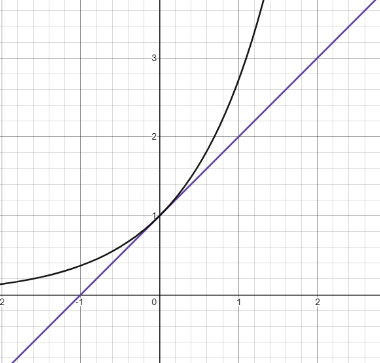
\includegraphics[width=0.3\textwidth]{Figs/1+x_leq_e^x.png}
    \caption{$1 + x \leq e^x$}
\end{figure}


% * * * * * * * * * * * * * * * * * * * * * * * * 
% * * * * * * * * * * * * * * * * * * * * * * * * 
% * * * * * * * * * * * * * * * * * * * * * * * * 
% * * * * * * * * * * * * * * * * * * * * * * * * 
% * * * * * * * * * * * * * * * * * * * * * * * * 
% * * * * * * * * * * * * * * * * * * * * * * * * 
% * * * * * * * * * * * * * * * * * * * * * * * * 
% * * * * * * * * * * * * * * * * * * * * * * * * 
% * * * * * * * * * * * * * * * * * * * * * * * * 
% * * * * * * * * * * * * * * * * * * * * * * * * 
% * * * * * * * * * * * * * * * * * * * * * * * * 
% * * * * * * * * * * * * * * * * * * * * * * * * 
% * * * * * * * * * * * * * * * * * * * * * * * * 
% * * * * * * * * * * * * * * * * * * * * * * * * 
% * * * * * * * * * * * * * * * * * * * * * * * * 
% * * * * * * * * * * * * * * * * * * * * * * * * 
% * * * * * * * * * * * * * * * * * * * * * * * * 
% * * * * * * * * * * * * * * * * * * * * * * * * 
% * * * * * * * * * * * * * * * * * * * * * * * * 



% * * * * * * * * * * * * * * * * * * * * * * * * 
% * * * * * * * * * * * * * * * * * * * * * * * * 
% * * * * * * * * * * * * * * * * * * * * * * * * 
% * * * * * * * * * * * * * * * * * * * * * * * * 
% * * * * * * * * * * * * * * * * * * * * * * * * 
% * * * * * * * * * * * * * * * * * * * * * * * * 
% * * * * * * * * * * * * * * * * * * * * * * * * 
% * * * * * * * * * * * * * * * * * * * * * * * * 
% * * * * * * * * * * * * * * * * * * * * * * * * 
% * * * * * * * * * * * * * * * * * * * * * * * * 
% * * * * * * * * * * * * * * * * * * * * * * * * 
% * * * * * * * * * * * * * * * * * * * * * * * * 
% * * * * * * * * * * * * * * * * * * * * * * * * 
% * * * * * * * * * * * * * * * * * * * * * * * * 
% * * * * * * * * * * * * * * * * * * * * * * * * 
% * * * * * * * * * * * * * * * * * * * * * * * * 
% * * * * * * * * * * * * * * * * * * * * * * * * 
% * * * * * * * * * * * * * * * * * * * * * * * * 
% * * * * * * * * * * * * * * * * * * * * * * * * 

\end{document}